\chapter{The best-practice estimate}
\label{chap:six}
% grammar checked (07-26)

In this chapter, I would like to focus on one other method that can be used to gain more insight into the effect's behavior. The technique in question involves utilizing the \ac{BMA} model coefficients from \autoref{chap:five} and actual data values to obtain a best-practice estimate of the effect under different specifications. With this, I hope first to uncover more detail about how different experiment setups change the observed effect and second to bring even more insight into the question of individual variables and the magnitude of their influence on the effect.


\section{Modelling the best-practice}
\label{sec:best_practice_base}

With the \ac{BMA} model coefficients from \autoref{tab:BMA}, let us first model a baseline subjective practice by plugging in mostly arbitrary data values. Once this subjective best-practice is obtained, we can then compare it to individual setups of other studies. Regarding the values used for the subjective evaluation, I opt to keep most of them at their mean. It is unclear and, at times, impossible to objectively discern between one and another value of a variable and say which is better. There are, however, two notable exceptions. First, I set the standard error equal to zero, as publication bias is never desirable in the data sample. Second, I utilize the highest available values of the journal impact factor and number of citations available. This stems from the assumption that highly cited studies from top journals should bring more credibility and present estimates close to the true effect.

Apart from this subjective best-practice estimate, I also computed best-practice estimates for all other studies in the dataset. When doing so, an important question arose of which specifications to use in case a study reported multiple estimates. To align with the idea of the best practice in the literature, the values chosen from each study as \textit{representative} should adhere to the specifications outlined in the previous paragraph as much as possible. For example, I mentioned that the standard error should be set to zero in the computation, as publication bias is generally undesirable. I will carry over this strong restrictions into the computation and set standard error to zero for all other studies as well. In regards to more lenient restrictions, such as using the maximum value of a variable, I will choose as representative the value from among the actual values reported in the study. If, say, a study reports the highest achieved education as 12 years, I will use that value as the representative, even if the study also reports the number of years of education as 10.

\begin{table}[!htbp]
  \centering
  \scriptsize
  \singlespace
  \caption{Implied best-practice}
  \label{tab:BPE_base}
  \begin{tabular}{
      @{}
      l
      *{3}{c}
      @{}}
    \toprule
    Study       & Estimate & 95\% Confidence Interval & Studies \\
    \midrule
    Author      & 6.536    & (5.762; 7.310)           & 0       \\
    Query       & 7.529    & (3.552; 11.506)          & 74      \\
    Snowballing & 6.346    & (2.530; 10.162)          & 41      \\
    All studies & 7.109    & (3.046; 11.17)           & 115     \\
    \bottomrule
    \multicolumn{4}{>{\scriptsize}p{0.6\linewidth}}{\emph{Note:} The table reports estimates of the best-practice estimate according to the author's subjective best-practice, two subsets of the literature, and the whole data sample. For the latter three, the figures are computed by averaging the best-practice estimates of all studies within that data subset. 95\% confidence interval bounds are constructed as an approximate using OLS with study level clustered standard errors. Query = Studies identified by query, Snowballing = Studies identified by snowballing, Studies = Number of studies used for the estimation.}
  \end{tabular}
\end{table}

As a baseline, I present the results of the implied best-practice calculation using my subjective setup. Then, I display estimates calculated across different subsets of literature for studies identified separately by the query and by the snowballing. Furthermore, I construct an estimate using all studies in the dataset. These can all be found in \autoref{tab:BPE_base}. The subjective best-practice estimate equals 6.5\% with a relatively narrow confidence band. The estimates for the two literature subsets then fall within 1\% of the subjective estimate; the query literature predicts a rate of 7.5\% returns to schooling, while the snowballing literature suggests 6.3\%. Understandably, the confidence bounds for these two estimates are much wider, given the large number of studies used in the estimation, together with the fact that this lumps together studies of a much different nature. Still, one could argue that the query studies tend to report higher estimates than their snowballing counterpart, although this claim would lack the statistical significance backup. When looking at the whole dataset, the suggested estimate tallies up to 7.1\% with a confidence bound much too wide to hold any statistical power. Despite this, I believe this number should serve, above all, as a good sanity check, and I think it does just that, given its proximity to the simple literature effect mean identified in \autoref{tab:sum}.

\section{Implied best-practice within subsets of literature}
\label{sec:best_practice_subsets}

To better understand how the implied best-practice behaves within the literature, I calculated how the estimates changed when observed for different data subsets. Using the same variable grouping logic described in \autoref{sec:best_practice_base}, I split the data into an array of subsets and present these in an intuitive graphical format. I choose this approach over focusing on individual studies as I believe it holds more information about individual variables' influence, but I append the best-practice estimates for all 115 studies in \autoref{app:four} for completeness.

Before getting to the actual results, several points about the technical procedure should be addressed, starting with a point on how the subsetting is done. Different variable types call for a different approach. In my data, I treated these different data types as follows. For dummy variables, the subset consists of studies where that dummy is equal to 0. For variables defined as ratios, such as the ratio of urban vs. rural workers, the subsets include studies where a given variable is the highest out of all its alternatives. For example, suppose that after choosing the most frequent values of the urban vs. rural workers variable, the ratio comes up to 0.25 vs. 0.75 (urban vs. rural). In that case, such a study gets put into the 'rural workers' category, given that these comprise the majority of the sample. The same is true for variables with multiple alternatives, such as for the variable capturing the highest achieved education. Suppose further that the ratio is the same for all variables of the same group. In that case, the representative is chosen randomly, eliminating potentially any bias given a large enough number of studies in the subset. Consequently, results from a sample containing fewer studies should be viewed with caution. And lastly, one note on handling float-type variables. Here, I use the median as the split point and divide the dataset into studies whose representative estimate is above and below this point.

% Another important caveat that this approach brings with it lies in using the most frequent value as the representative value for each study. Naturally, this procedure leads to a loss of information, skewing the overall statistics a bit as a result. For example, the number of citations median of the grouped sample of studies is no longer 80 as in the ungrouped dataset, but 73. As I mentioned in \autoref{sec:best_practice_base}, this could be remedied by weighting each variable with the number of occurrences within the reported estimates of each study. Personally, however, I consider the overall impact of this shortcoming minimal. Moreover, it could be argued that the best practice in literature is the one that each study tends to employ the most, but that, too, is up for debate.

The graphical results can be found in
\autoref{fig:bpe_graphs}. For presentation of clarity, I choose to omit several data subsets, and present only the ones that align with the focus of this work. With the formidable number of estimates included in each data subsample, I firmly believe the shown results accurately represent the overall behavior within the literature and that they paint a clear enough picture.

% BPE summary statistics
% \begin{table}[!htbp]
% \centering
% \scriptsize
% \singlespace
% \caption{Implied best-practice across various subsets of data}
% \label{tab:bpe_summary_stats}
% \begin{tabular}{
% @{}
% l % Description
% *{7}{c} % Middle columns
% >{\centering\arraybackslash}p{1cm} % Last column with fixed width
% @{}
% }
% \toprule
%     & Mean & \multicolumn{2}{c}{95\% conf. int.} & Median & Min & Max & SD & Studies \\

% \midrule

%                            All studies & 7.109 & 3.046   & 11.172  & 7.239 & 1.152 & 12.436 & 2.073 & 115 \\
%     \midrule

% \multicolumn{8}{l}{\emph{Data characteristics}}\\	
%      Yrs. of Schooling >= 10.6 & 6.907     & 3.199   & 10.615  & 6.749 & 3.503 & 11.598 & 1.892      & 59 \\
%       Yrs. of Schooling < 10.6 & 7.321     & 2.917   & 11.725  & 7.360 & 1.152 & 12.436 & 2.247      & 56 \\
%      Yrs. of Experience < 19.5 & 7.406     & 3.310   & 11.502  & 7.505 & 3.133 & 11.598 & 2.090      & 56 \\
%    Yrs. of Experience >= 19.45 & 6.826     & 2.837   & 10.815  & 6.790 & 1.152 & 12.436 & 2.035      & 59 \\
%               Education: Years & 7.119     & 3.181   & 11.057  & 7.134 & 1.152 & 12.436 & 2.009      & 84 \\
%              Education: Levels & 7.079     & 2.624   & 11.534  & 7.254 & 2.932 & 11.598 & 2.273      & 31 \\
%         National Register Data & 7.161     & 3.057   & 11.265  & 6.801 & 3.133 & 11.128 & 2.094      & 35 \\
%                     Micro Data & 7.484     & 4.313   & 10.655  & 7.573 & 4.168 & 11.146 & 1.618      & 18 \\
%                    Survey Data & 6.970     & 2.678   & 11.262  & 6.898 & 1.152 & 12.436 & 2.190      & 62 \\
%           Cross-sectional Data & 7.299     & 3.808   & 10.790  & 7.248 & 3.669 & 11.598 & 1.781      & 44 \\
%                     Panel Data & 6.991     & 2.601   & 11.381  & 6.979 & 1.152 & 12.436 & 2.240      & 71 \\
%               Higher Education & 7.729     & 3.380   & 12.078  & 7.463 & 3.745 & 11.598 & 2.219      & 23 \\
%            Secondary Education & 6.986     & 3.086   & 10.886  & 6.912 & 3.133 & 12.436 & 1.990      & 72 \\
%              Primary Education & 7.200     & 2.798   & 11.602  & 7.576 & 1.152 & 10.083 & 2.246      & 13 \\
%     \midrule

% \multicolumn{8}{l}{\emph{Spatial/structural variation}}\\
%                   No Education & 6.164     & 2.250   & 10.078  & 7.029 & 2.932  & 7.846 & 1.997       & 7 \\
%                   Wage Earners & 7.050     & 2.977   & 11.123  & 7.006 & 1.152 & 12.436 & 2.078     & 109 \\
%                  Self-Employed & 8.175     & 4.590   & 11.760  & 7.415 & 6.746 & 11.598 & 1.829       & 6 \\
%                   Gender: Male & 7.242     & 3.430   & 11.054  & 7.254 & 1.152 & 12.436 & 1.945      & 97 \\
%                 Gender: Female & 6.388     & 1.272   & 11.504  & 6.250 & 2.932 & 11.146 & 2.610      & 18 \\
%           Ethnicity: Caucasian & 6.907     & 3.650   & 10.164  & 6.749 & 4.015 & 11.146 & 1.662      & 31 \\
%               Ethnicity: Other & 7.183     & 2.851   & 11.515  & 7.360 & 1.152 & 12.436 & 2.210      & 84 \\
%                  Sector: Urban & 7.077     & 2.943   & 11.211  & 7.123 & 1.152 & 11.598 & 2.109     & 102 \\
%                  Sector: Rural & 7.353     & 3.782   & 10.924  & 7.256 & 5.191 & 12.436 & 1.822      & 13 \\
%                   Income: High & 7.192     & 3.684   & 10.700  & 6.912 & 3.745 & 11.261 & 1.790      & 60 \\
%                 Income: Middle & 7.077     & 2.414   & 11.740  & 7.368 & 1.152 & 12.436 & 2.379      & 48 \\
%                    Income: Low & 6.606     & 2.029   & 11.183  & 6.115 & 2.932 & 10.083 & 2.335       & 7 \\
%     Median Expenditure >= 8477 & 6.981     & 3.079   & 10.883  & 6.749 & 1.152 & 11.261 & 1.991      & 62 \\
%      Median Expenditure < 8477 & 7.258     & 2.993   & 11.523  & 7.319 & 3.133 & 12.436 & 2.176      & 53 \\
%             Minimum Wage < 345 & 6.976     & 2.860   & 11.092  & 7.282 & 1.152 & 12.436 & 2.100      & 57 \\
%            Minimum Wage >= 345 & 7.239     & 3.207   & 11.271  & 6.822 & 3.503 & 11.598 & 2.057      & 58 \\
%                 Mean Age >= 37 & 6.863     & 3.335   & 10.391  & 6.770 & 2.932 & 11.232 & 1.800      & 60 \\
%                  Mean Age < 37 & 7.377     & 2.824   & 11.930  & 7.402 & 1.152 & 12.436 & 2.323      & 55 \\
%                  \midrule

% \multicolumn{8}{l}{\emph{Estimation method}}\\  
%                    Method: OLS & 7.270     & 3.070   & 11.470  & 7.282 & 1.152 & 12.436 & 2.143      & 85 \\
%                   Method: 2SLS & 7.153     & 3.096   & 11.210  & 6.993 & 3.683 & 10.767 & 2.070       & 8 \\
%                Method: Heckman & 6.417     & 2.824   & 10.010  & 5.434 & 5.286  & 8.532 & 1.833       & 3 \\
%                     Method: IV & 6.774     & 3.223   & 10.325  & 7.029 & 4.015 & 10.424 & 1.812      & 11 \\
%              Method: Cohort/FE & 5.861     & 2.388    & 9.334  & 5.974 & 3.503  & 8.476 & 1.772       & 7 \\
%                 Method: Probit & 7.541        & NA       & NA  & 7.541 & 7.541  & 7.541    & NA       & 1 \\
%               Ability: Proxied & 6.729    & 2.531   & 10.927  & 7.006 & 2.932 & 11.232 & 2.142  &      23 \\
%           Ability: Unmentioned & 7.134    & 4.057   & 10.211  & 6.979 & 3.712 & 10.767 & 1.570  &      29 \\
%          Ability: Uncontrolled & 7.312    & 3.155   & 11.469  & 7.300 & 1.152 & 12.436 & 2.121  &      52 \\
%                Ability: Direct & 6.873    & 1.173   & 12.573  & 5.580 & 3.503 & 11.598 & 2.908  &      11 \\
%                    \midrule

% \multicolumn{8}{l}{\emph{Publication characteristics}}\\  
%         Impact Factor >= 0.222 & 7.066    & 3.270   & 10.862  & 6.890 & 3.503 & 12.436 & 1.937  &      58 \\
%          Impact Factor < 0.222 & 7.152    & 2.801   & 11.503  & 7.319 & 1.152 & 11.598 & 2.220  &      57 \\
%                Citations >= 73 & 7.130    & 3.453   & 10.807  & 7.134 & 3.656 & 11.261 & 1.876  &      58 \\
%                 Citations < 73 & 7.086    & 2.631   & 11.541  & 7.254 & 1.152 & 12.436 & 2.273  &      57 \\
%               Study: Published & 7.244    & 3.261   & 11.227  & 7.254 & 3.133 & 12.436 & 2.032  &      93 \\
%             Study: Unpublished & 6.535    & 2.227   & 10.843  & 6.749 & 1.152 & 11.146 & 2.198  &      22 \\

%     \bottomrule                                               

% \multicolumn{9}{>{\scriptsize}p{0.95\linewidth}}{\emph{Note:} This table displays implied best practice across the whole literature sample across different subsets of the main data. For determining the value of variables for each study, mode is used. For cutoff points of numeric, non-ratio type variables, medians are used. SD = Standard Deviation, OLS = Ordinary Least Squares, 2SLS = Two-stage Least Squares, IV = Instrumental Variable, FE = Fixed-Effects.}
% \end{tabular}
% \end{table}


% BPE graphs
%Education: years/levels
%Data type: panel/cross
%Highest achieved education
%Male vs female
%Income: high, low, middle
%Methods, 
%Ability, 
%Citations
\begin{figure}[!htbp]
  \begin{center}
    \caption{Implied best-practice across various subsets of data}
    \label{fig:bpe_graphs}

    \begin{subfigure}[!htbp]{0.38\textwidth}
      \vspace{-0.1cm}
      \caption{Education type}
      \vspace{-0.1cm}
      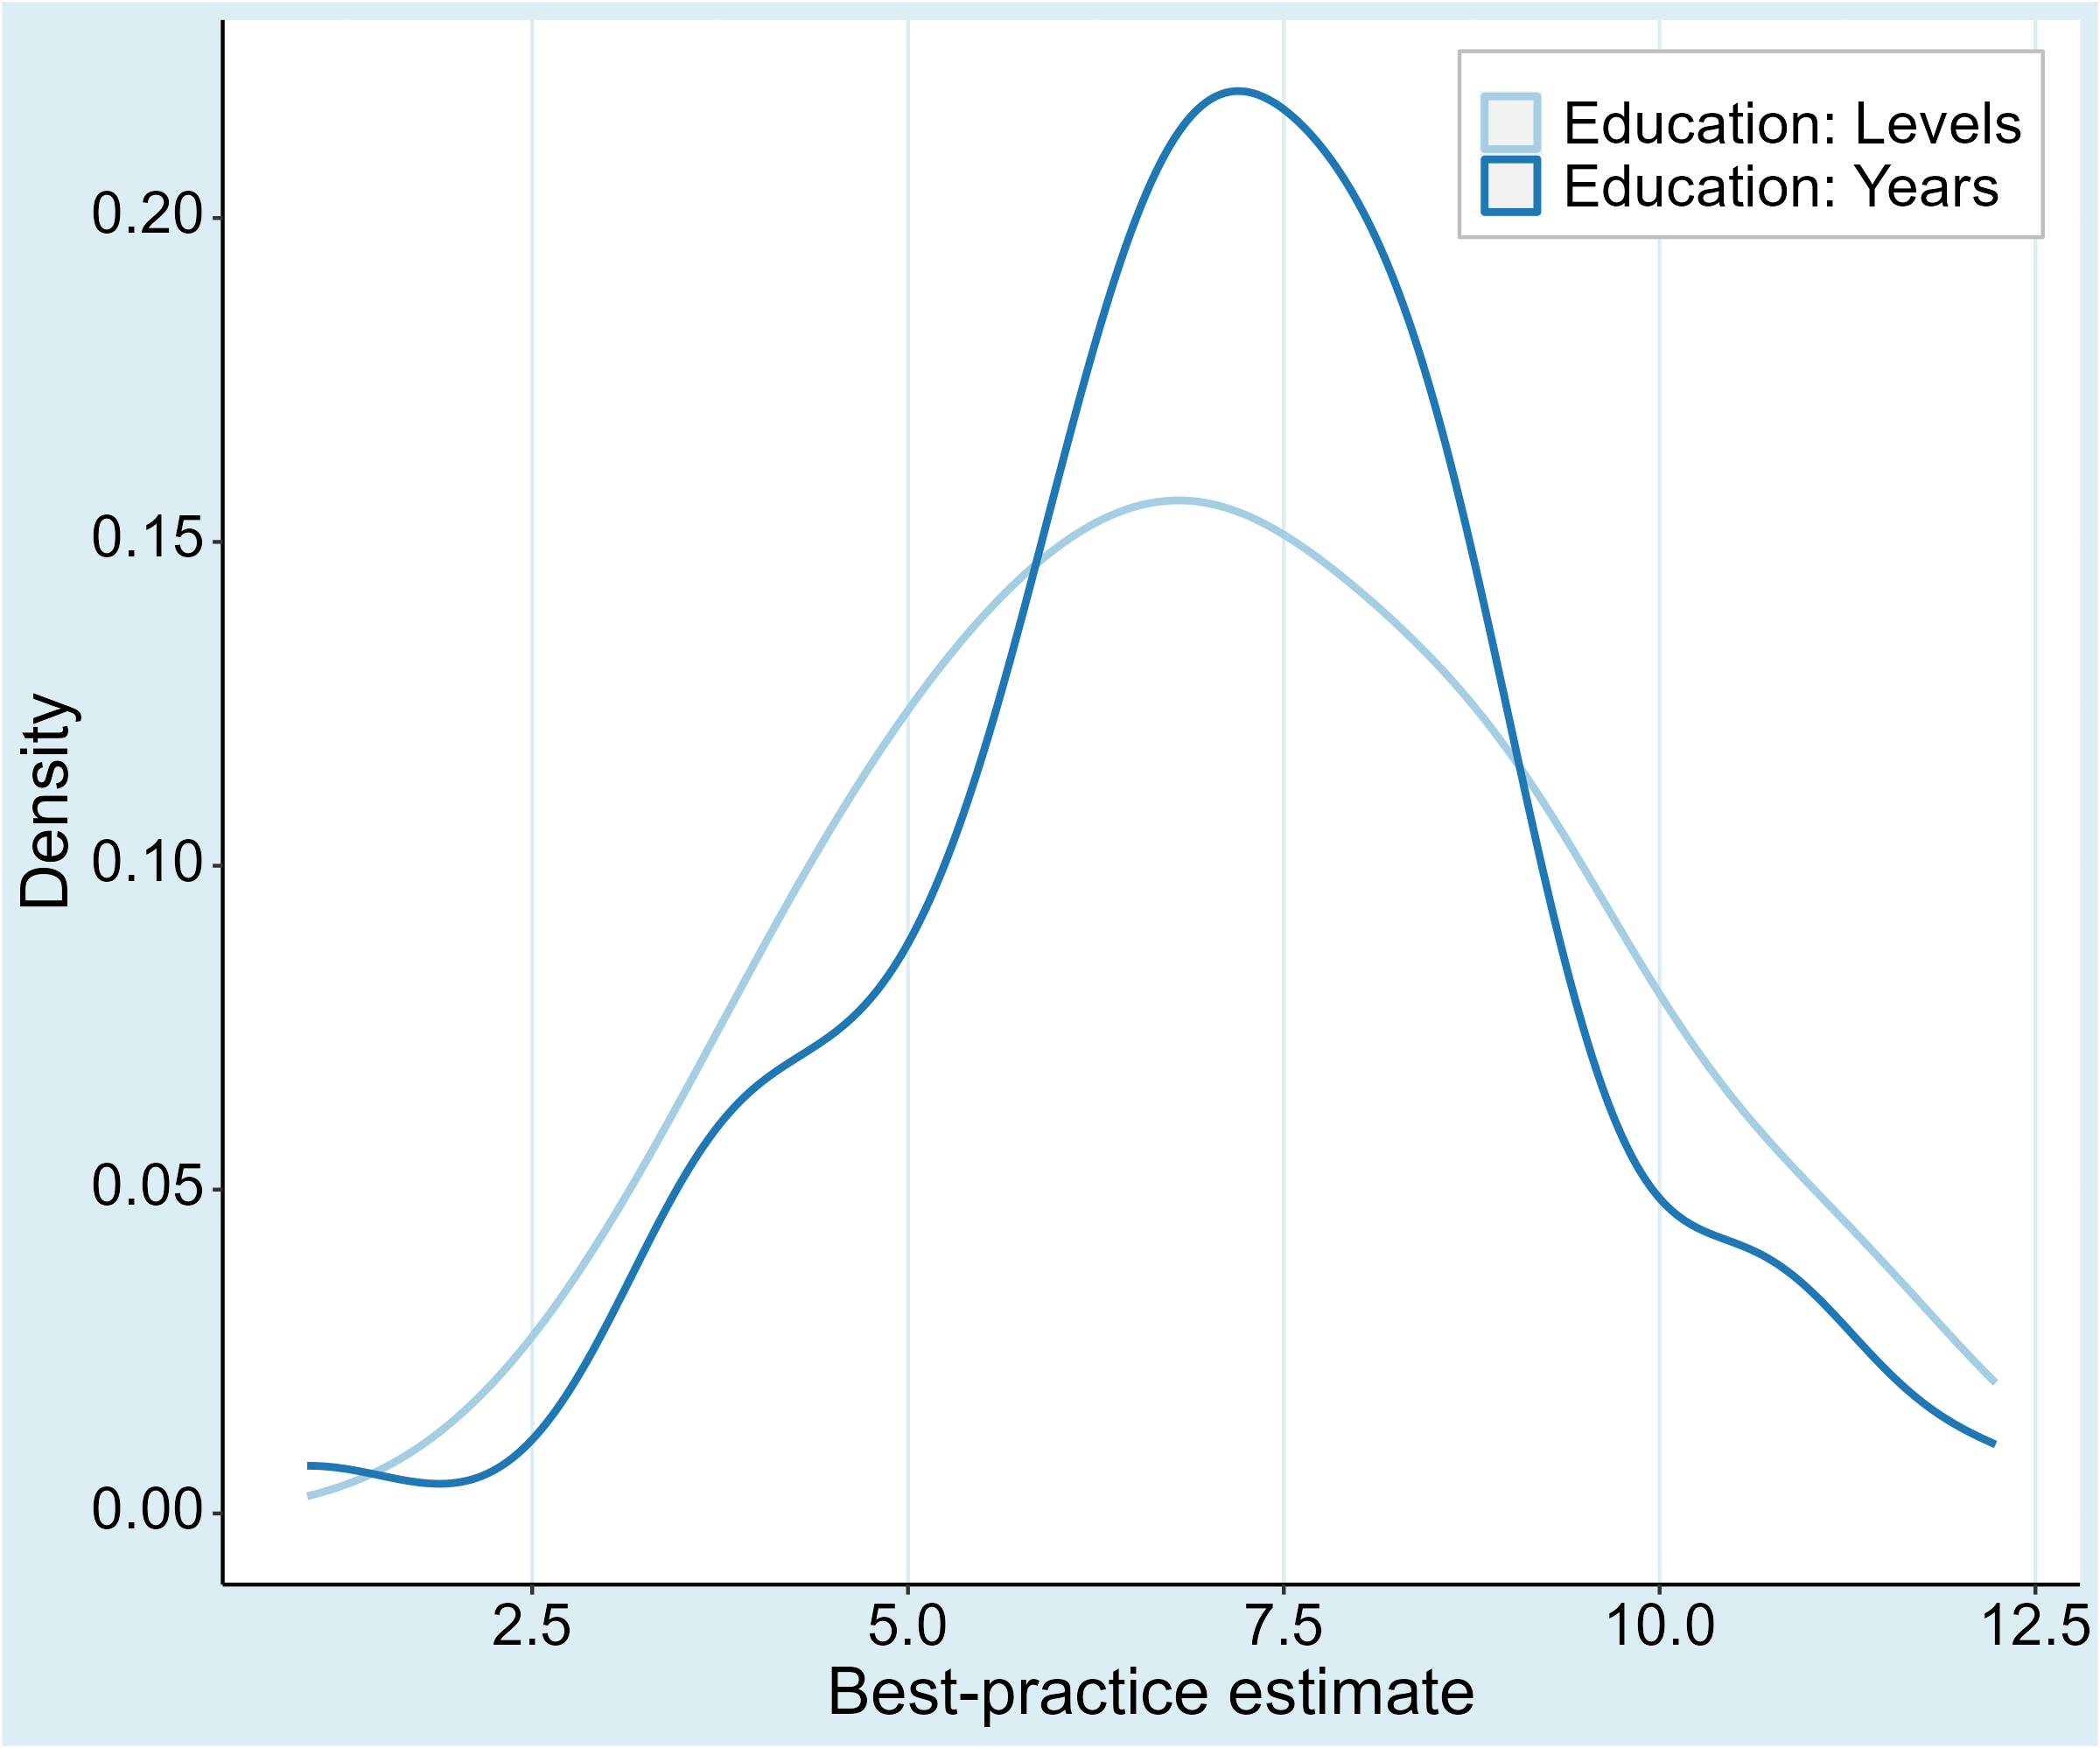
\includegraphics[width=0.95\linewidth]{Figures/BPE/bpe_years_levels.png}
      \label{fig:bpe_years_levels}
    \end{subfigure}
    \begin{subfigure}[!htbp]{0.38\textwidth}
      \vspace{-0.1cm}
      \caption{Data type}
      \vspace{-0.1cm}
      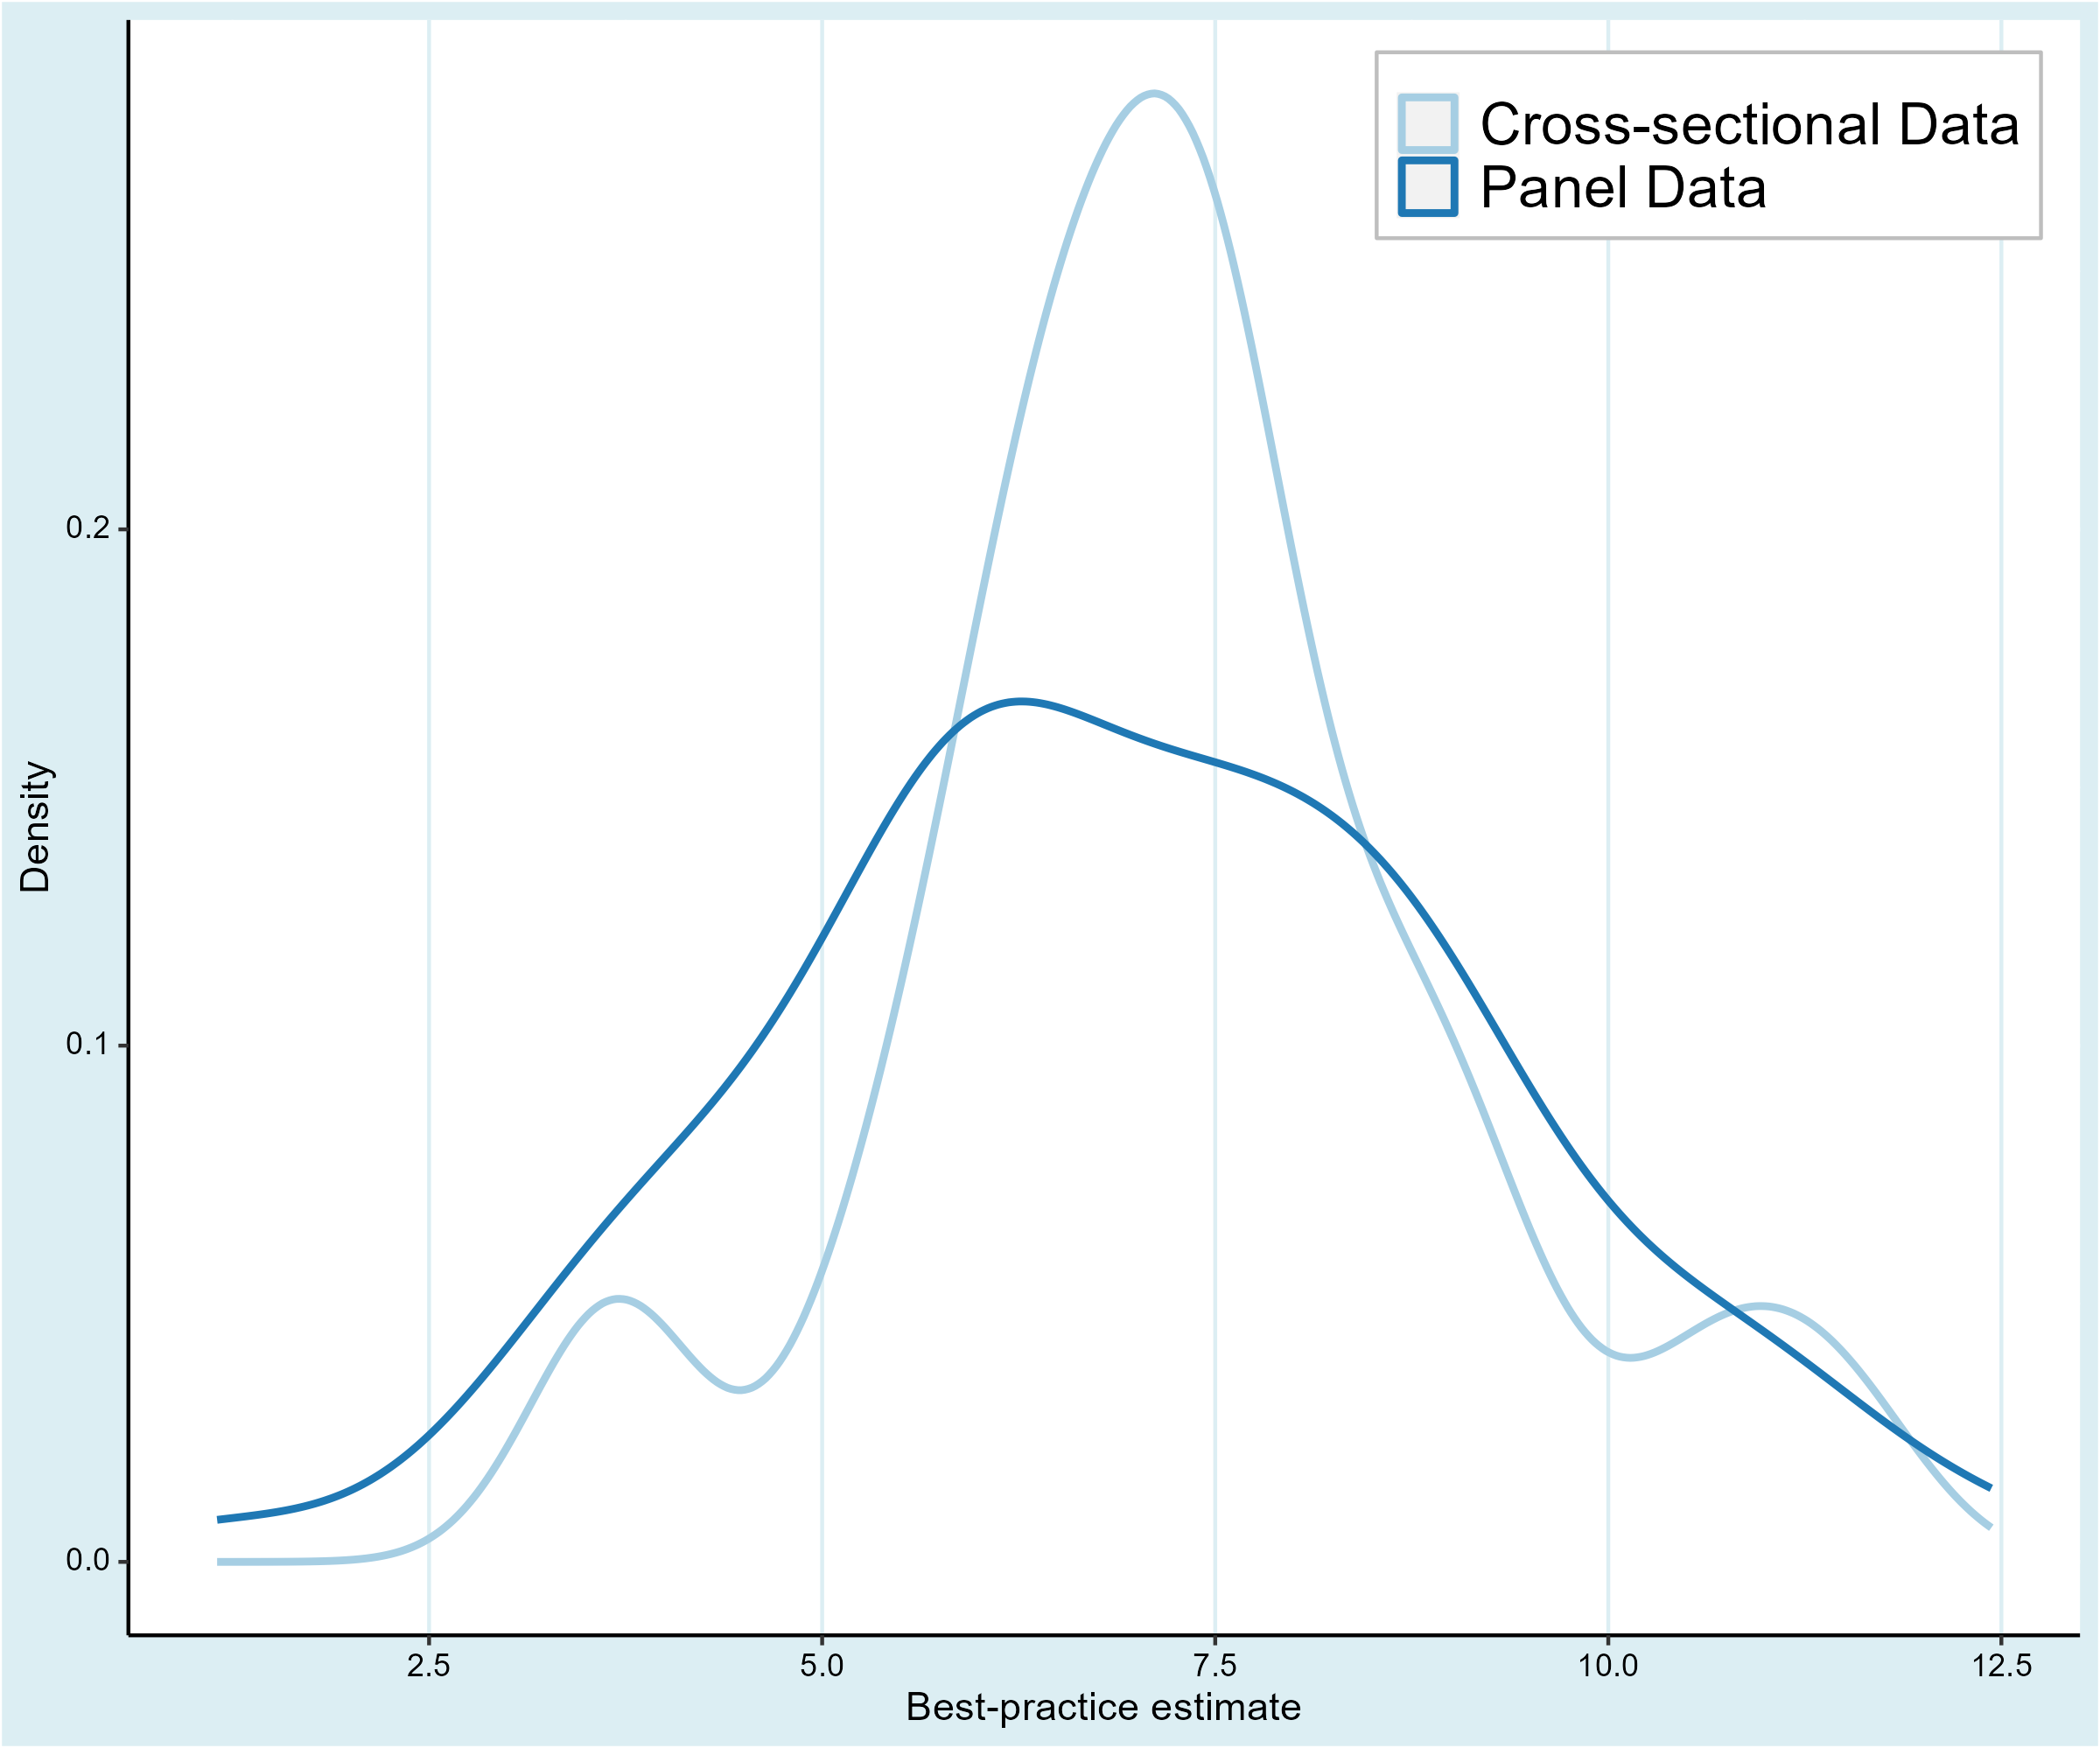
\includegraphics[width=0.95\linewidth]{Figures/BPE/bpe_data_type.png}
      \label{fig:bpe_data_type}
    \end{subfigure}

    \begin{subfigure}[!htbp]{0.38\textwidth}
      \vspace{0.2cm}
      \caption{Highest education}
      \vspace{-0.1cm}
      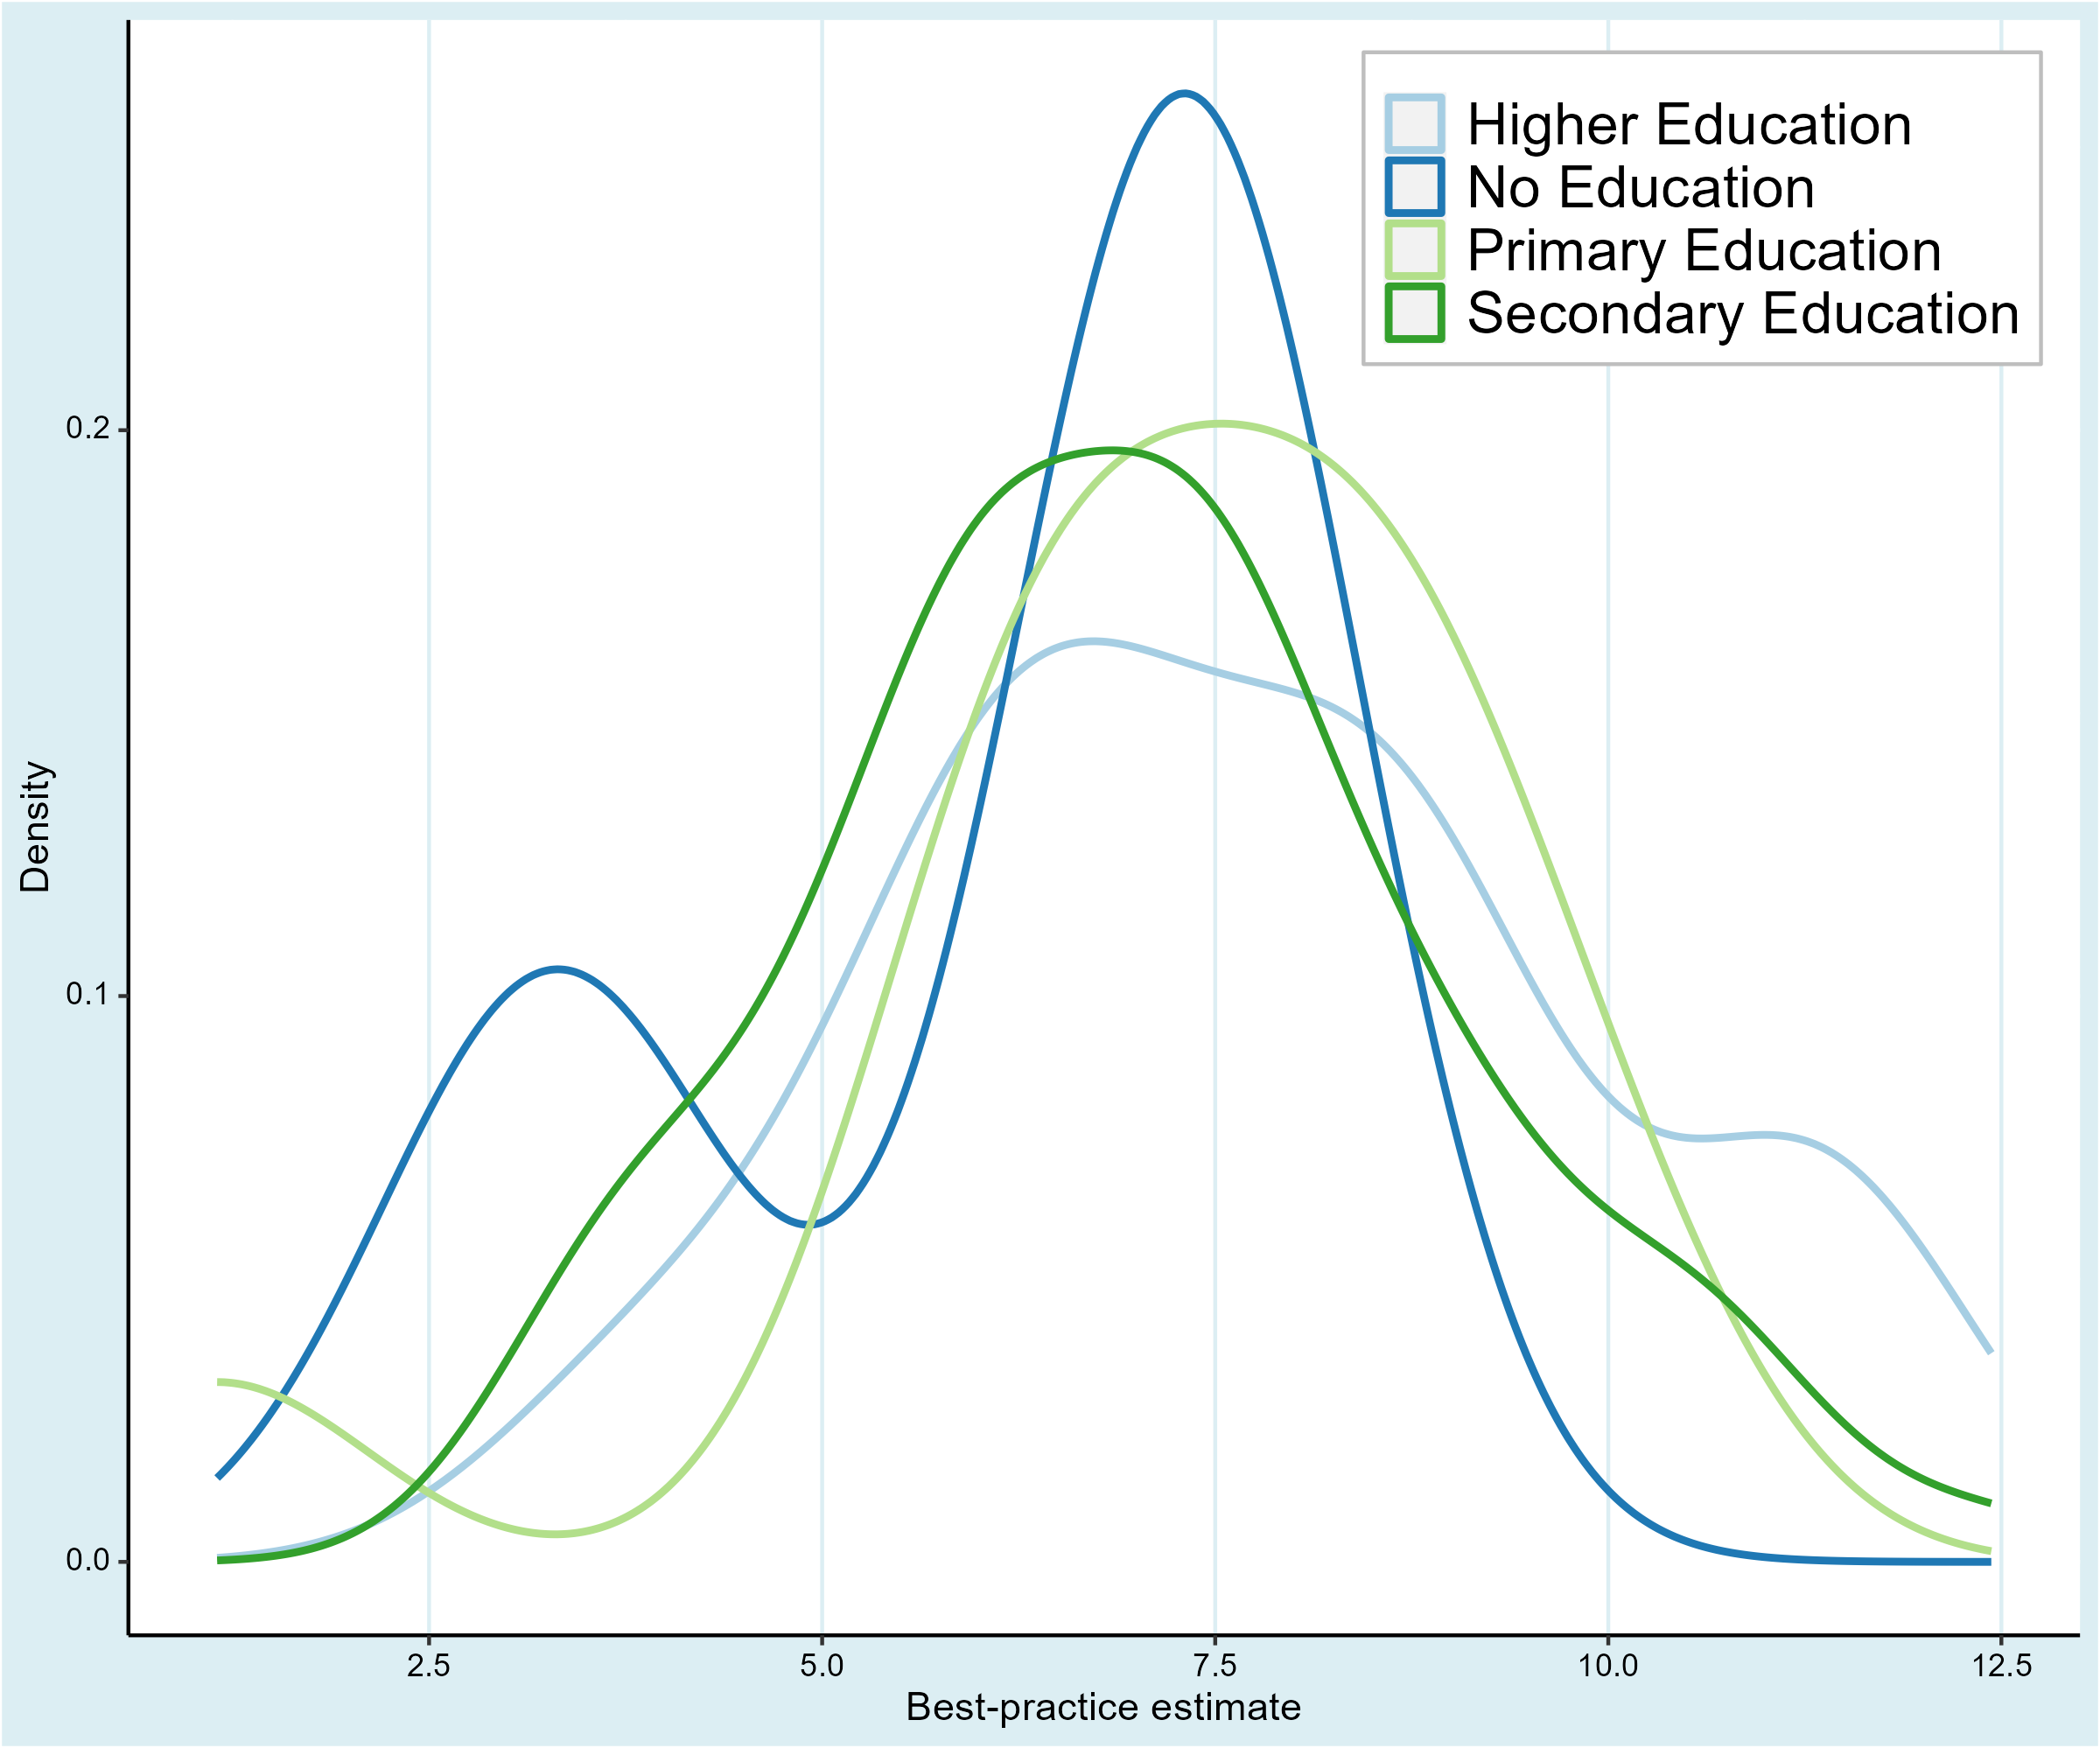
\includegraphics[width=0.95\linewidth]{Figures/BPE/bpe_education.png}
      \label{fig:bpe_education}
    \end{subfigure}
    \begin{subfigure}[!htbp]{0.38\textwidth}
      \vspace{0.2cm}
      \caption{Gender}
      \vspace{-0.1cm}
      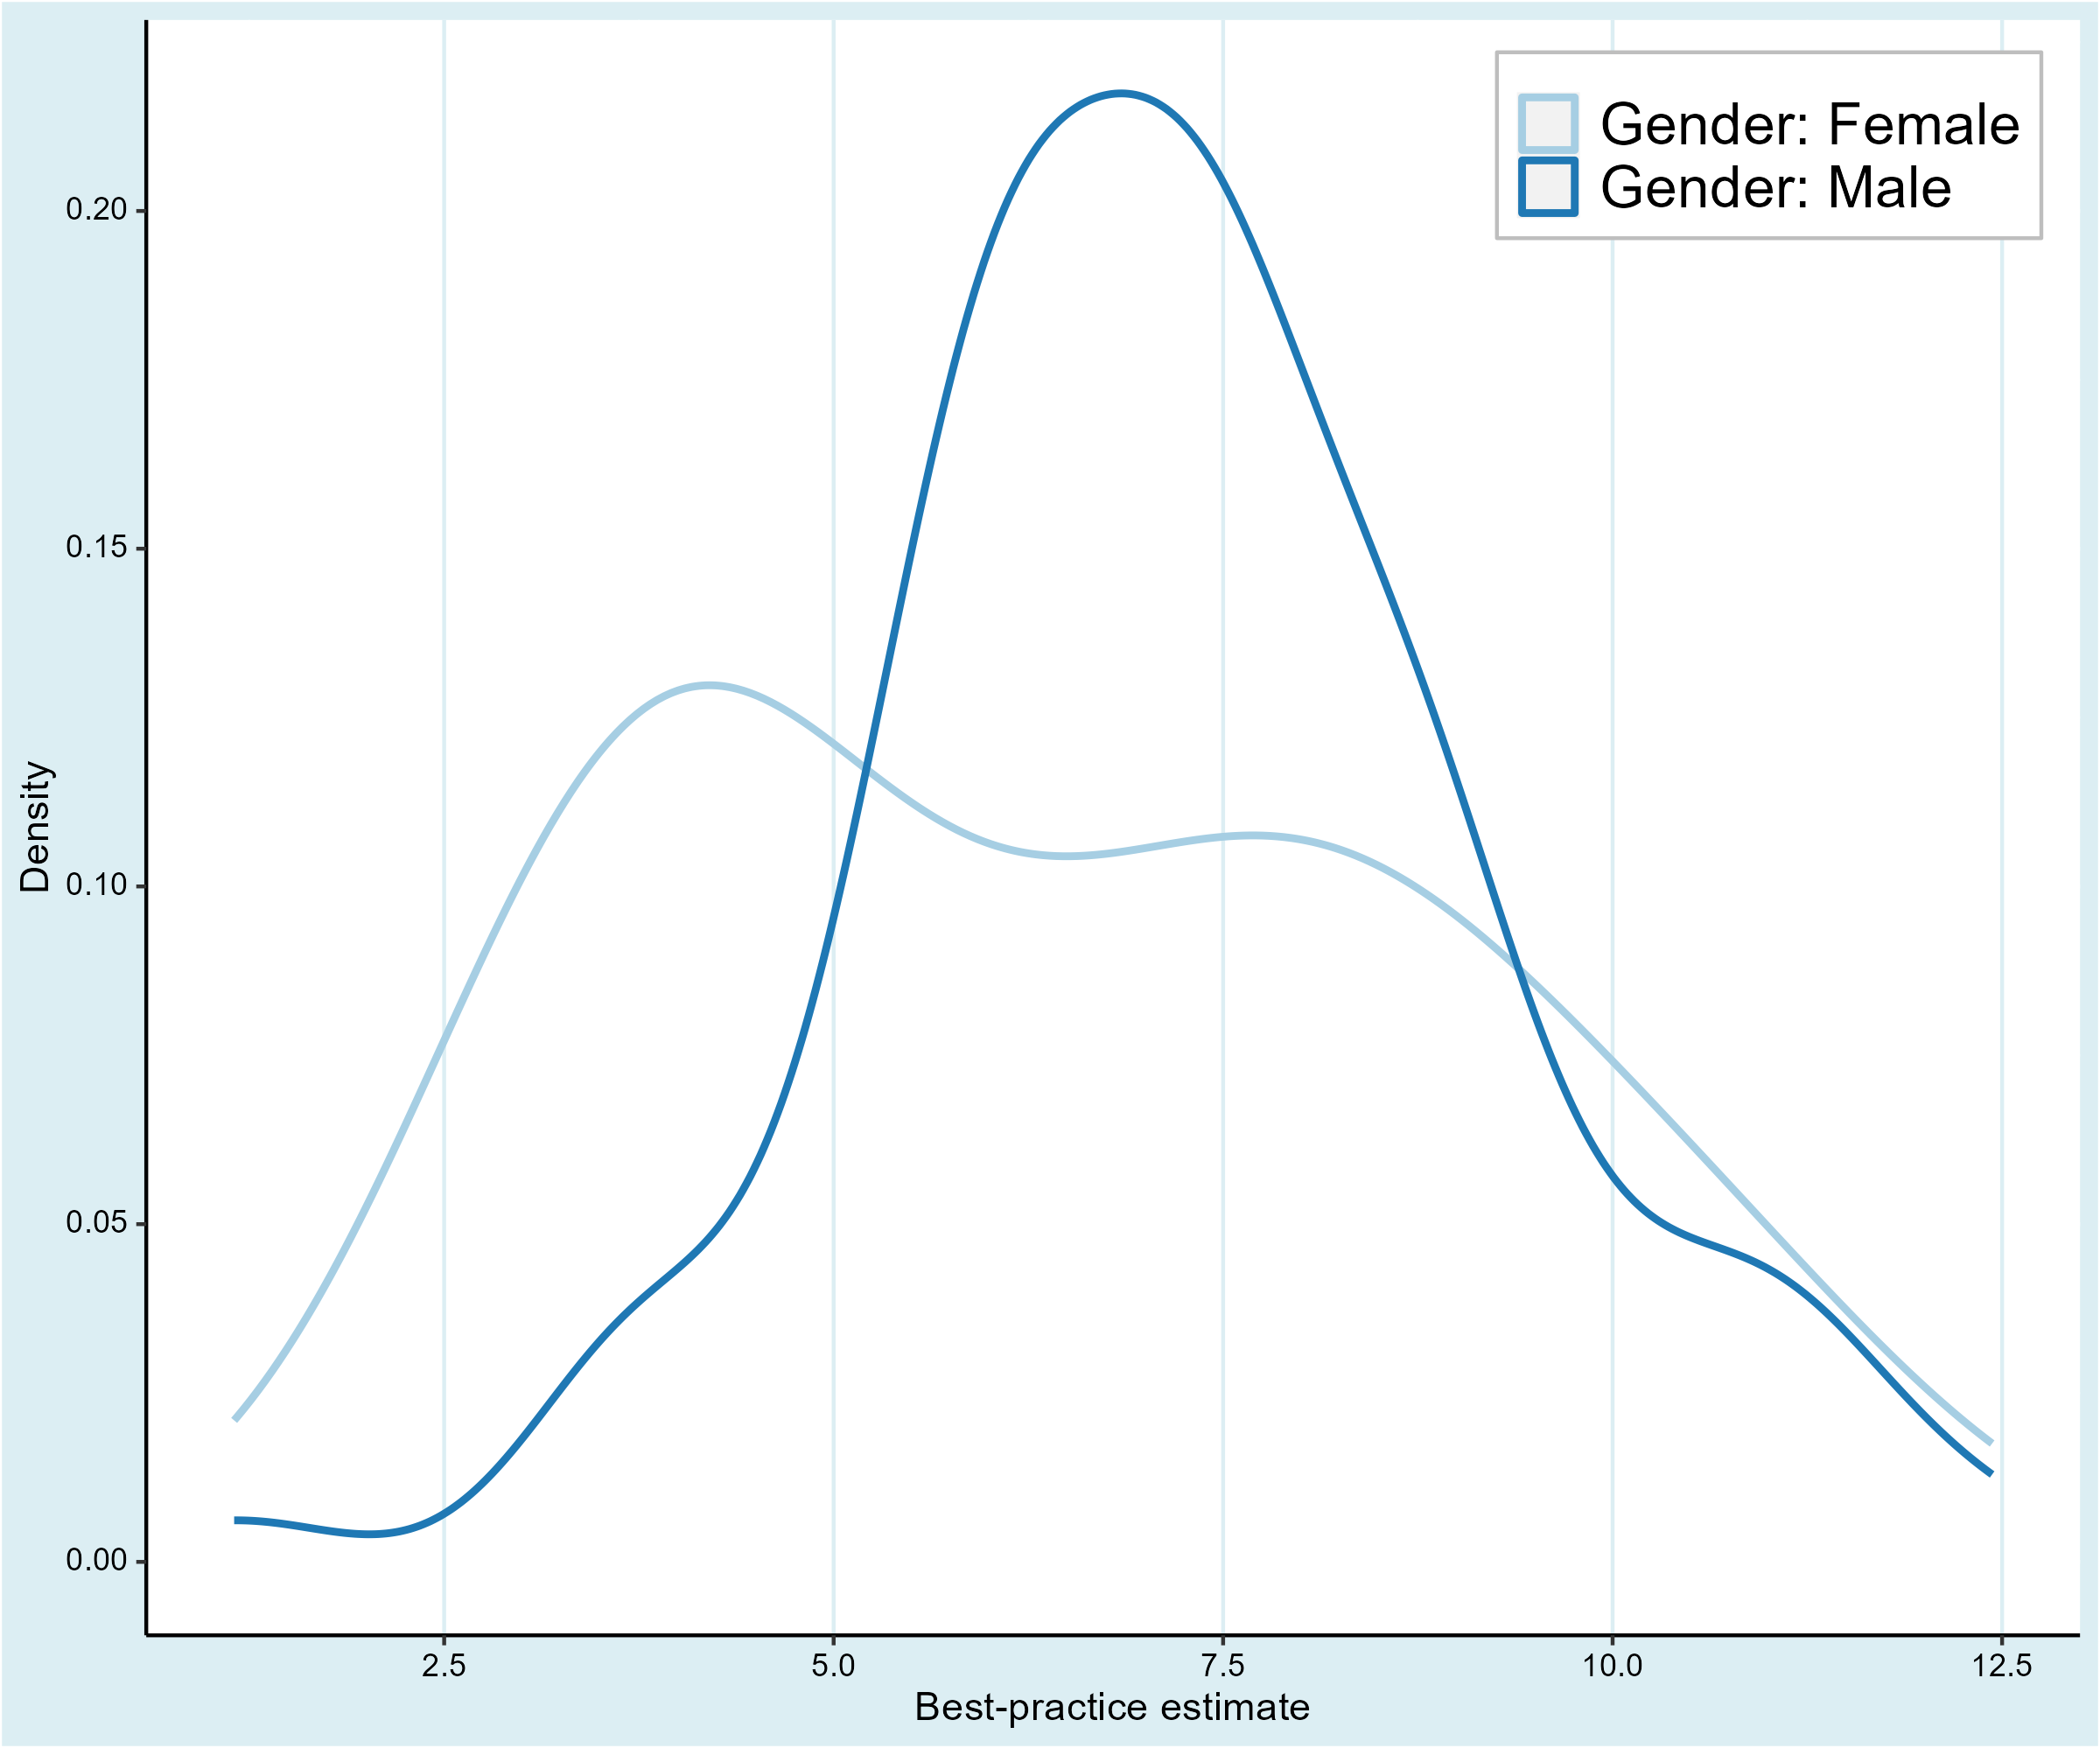
\includegraphics[width=0.95\linewidth]{Figures/BPE/bpe_gender.png}
      \label{fig:bpe_gender}
    \end{subfigure}

    \begin{subfigure}[!htbp]{0.38\textwidth}
      \vspace{0.2cm}
      \caption{Country wealth}
      \vspace{-0.1cm}
      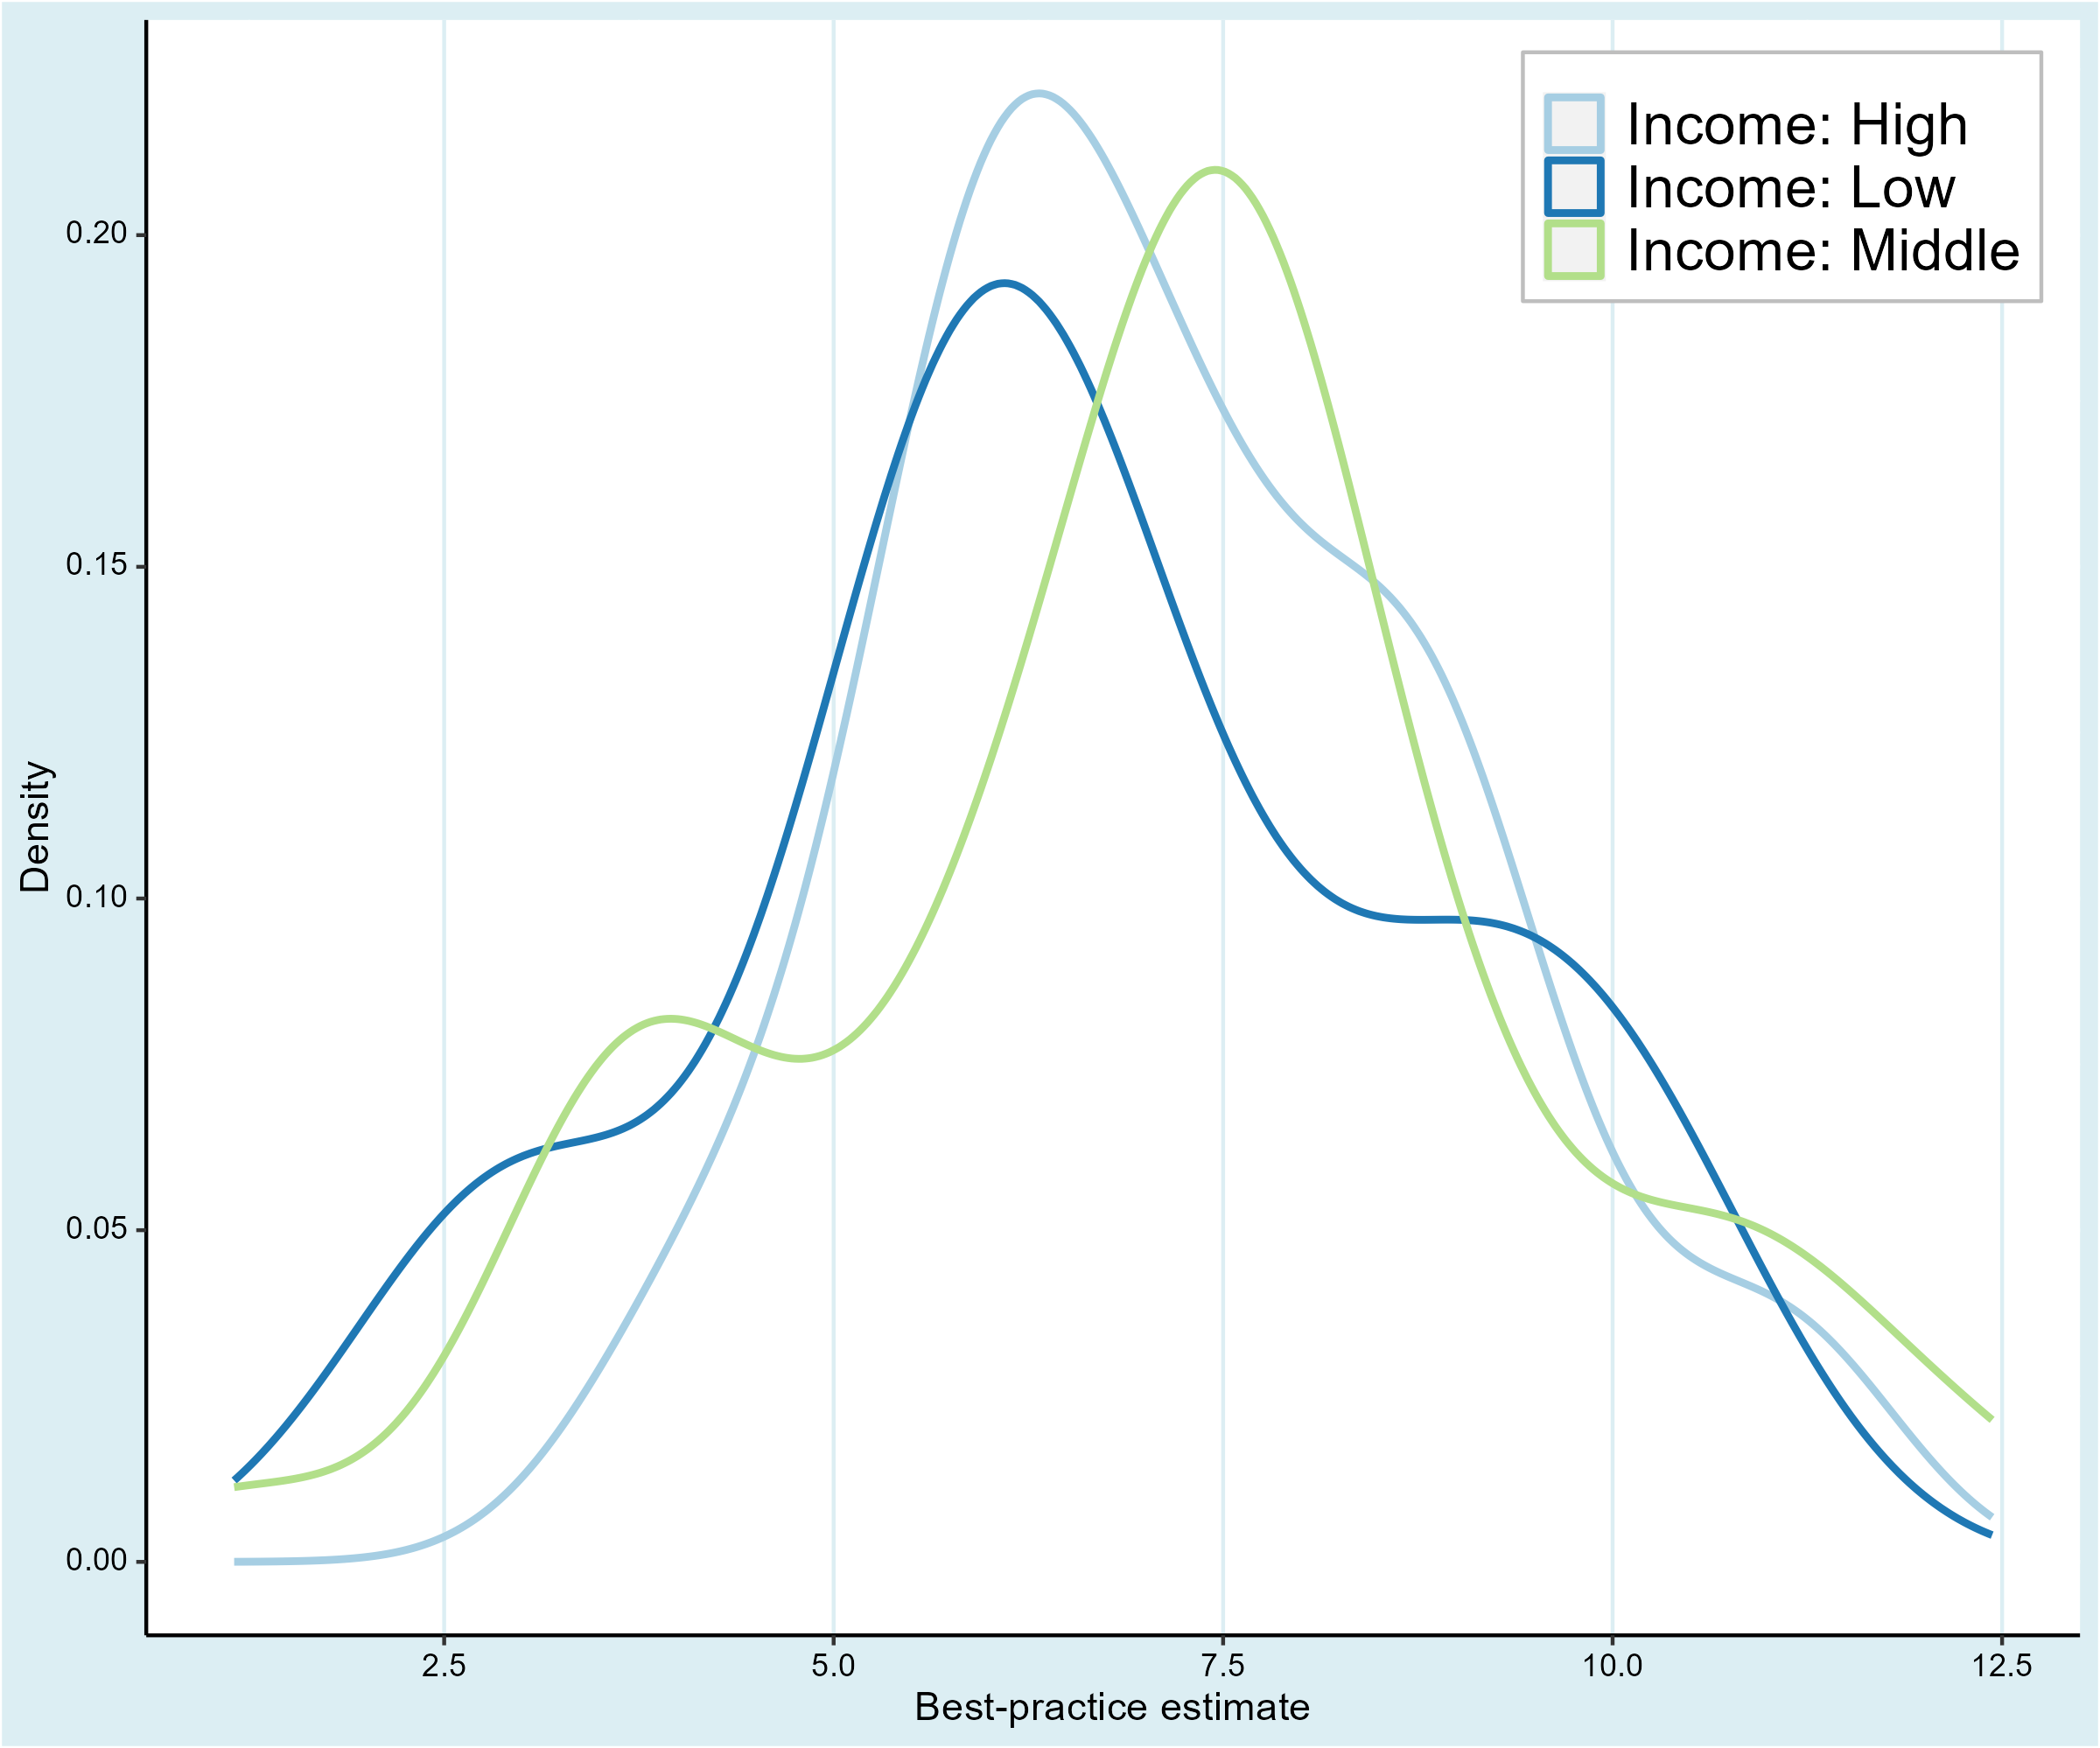
\includegraphics[width=0.95\linewidth]{Figures/BPE/bpe_income.png}
      \label{fig:bpe_income}
    \end{subfigure}
    \begin{subfigure}[!htbp]{0.38\textwidth}
      \vspace{0.2cm}
      \caption{Estimation method}
      \vspace{-0.1cm}
      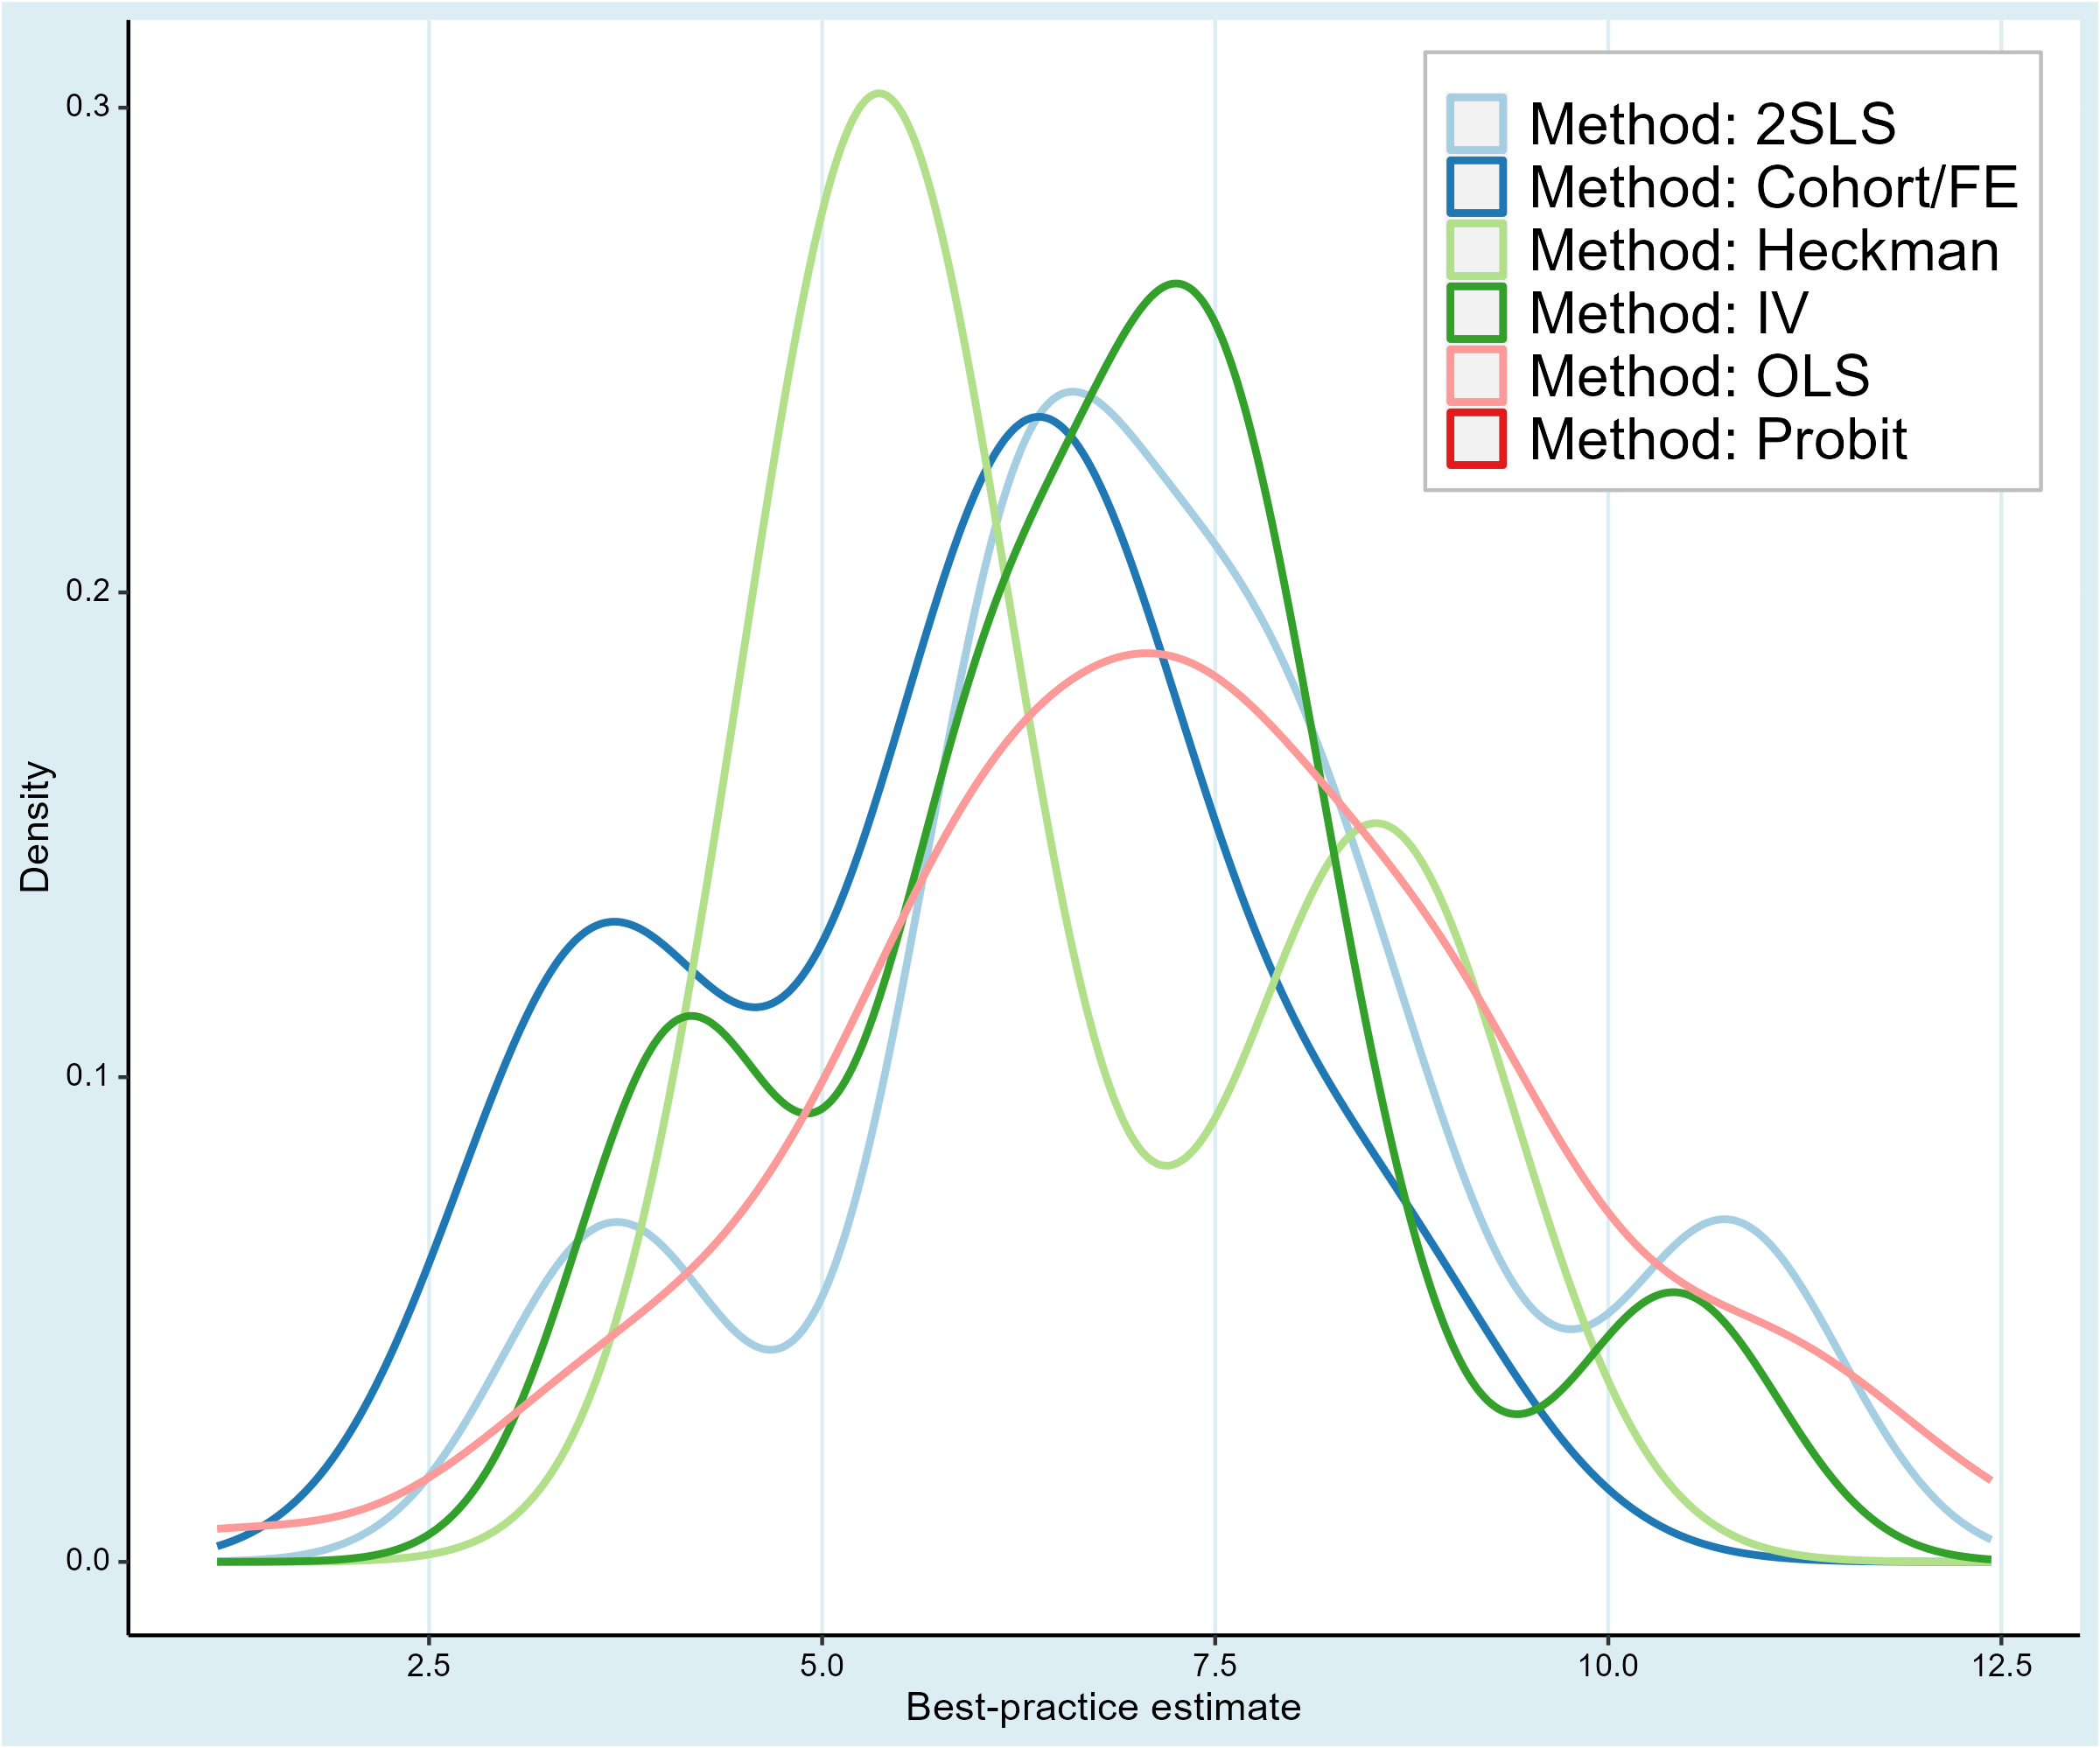
\includegraphics[width=0.95\linewidth]{Figures/BPE/bpe_method.png}
      \label{fig:bpe_method}
    \end{subfigure}

    \begin{subfigure}[!htbp]{0.38\textwidth}
      \vspace{0.2cm}
      \caption{Ability}
      \vspace{-0.1cm}
      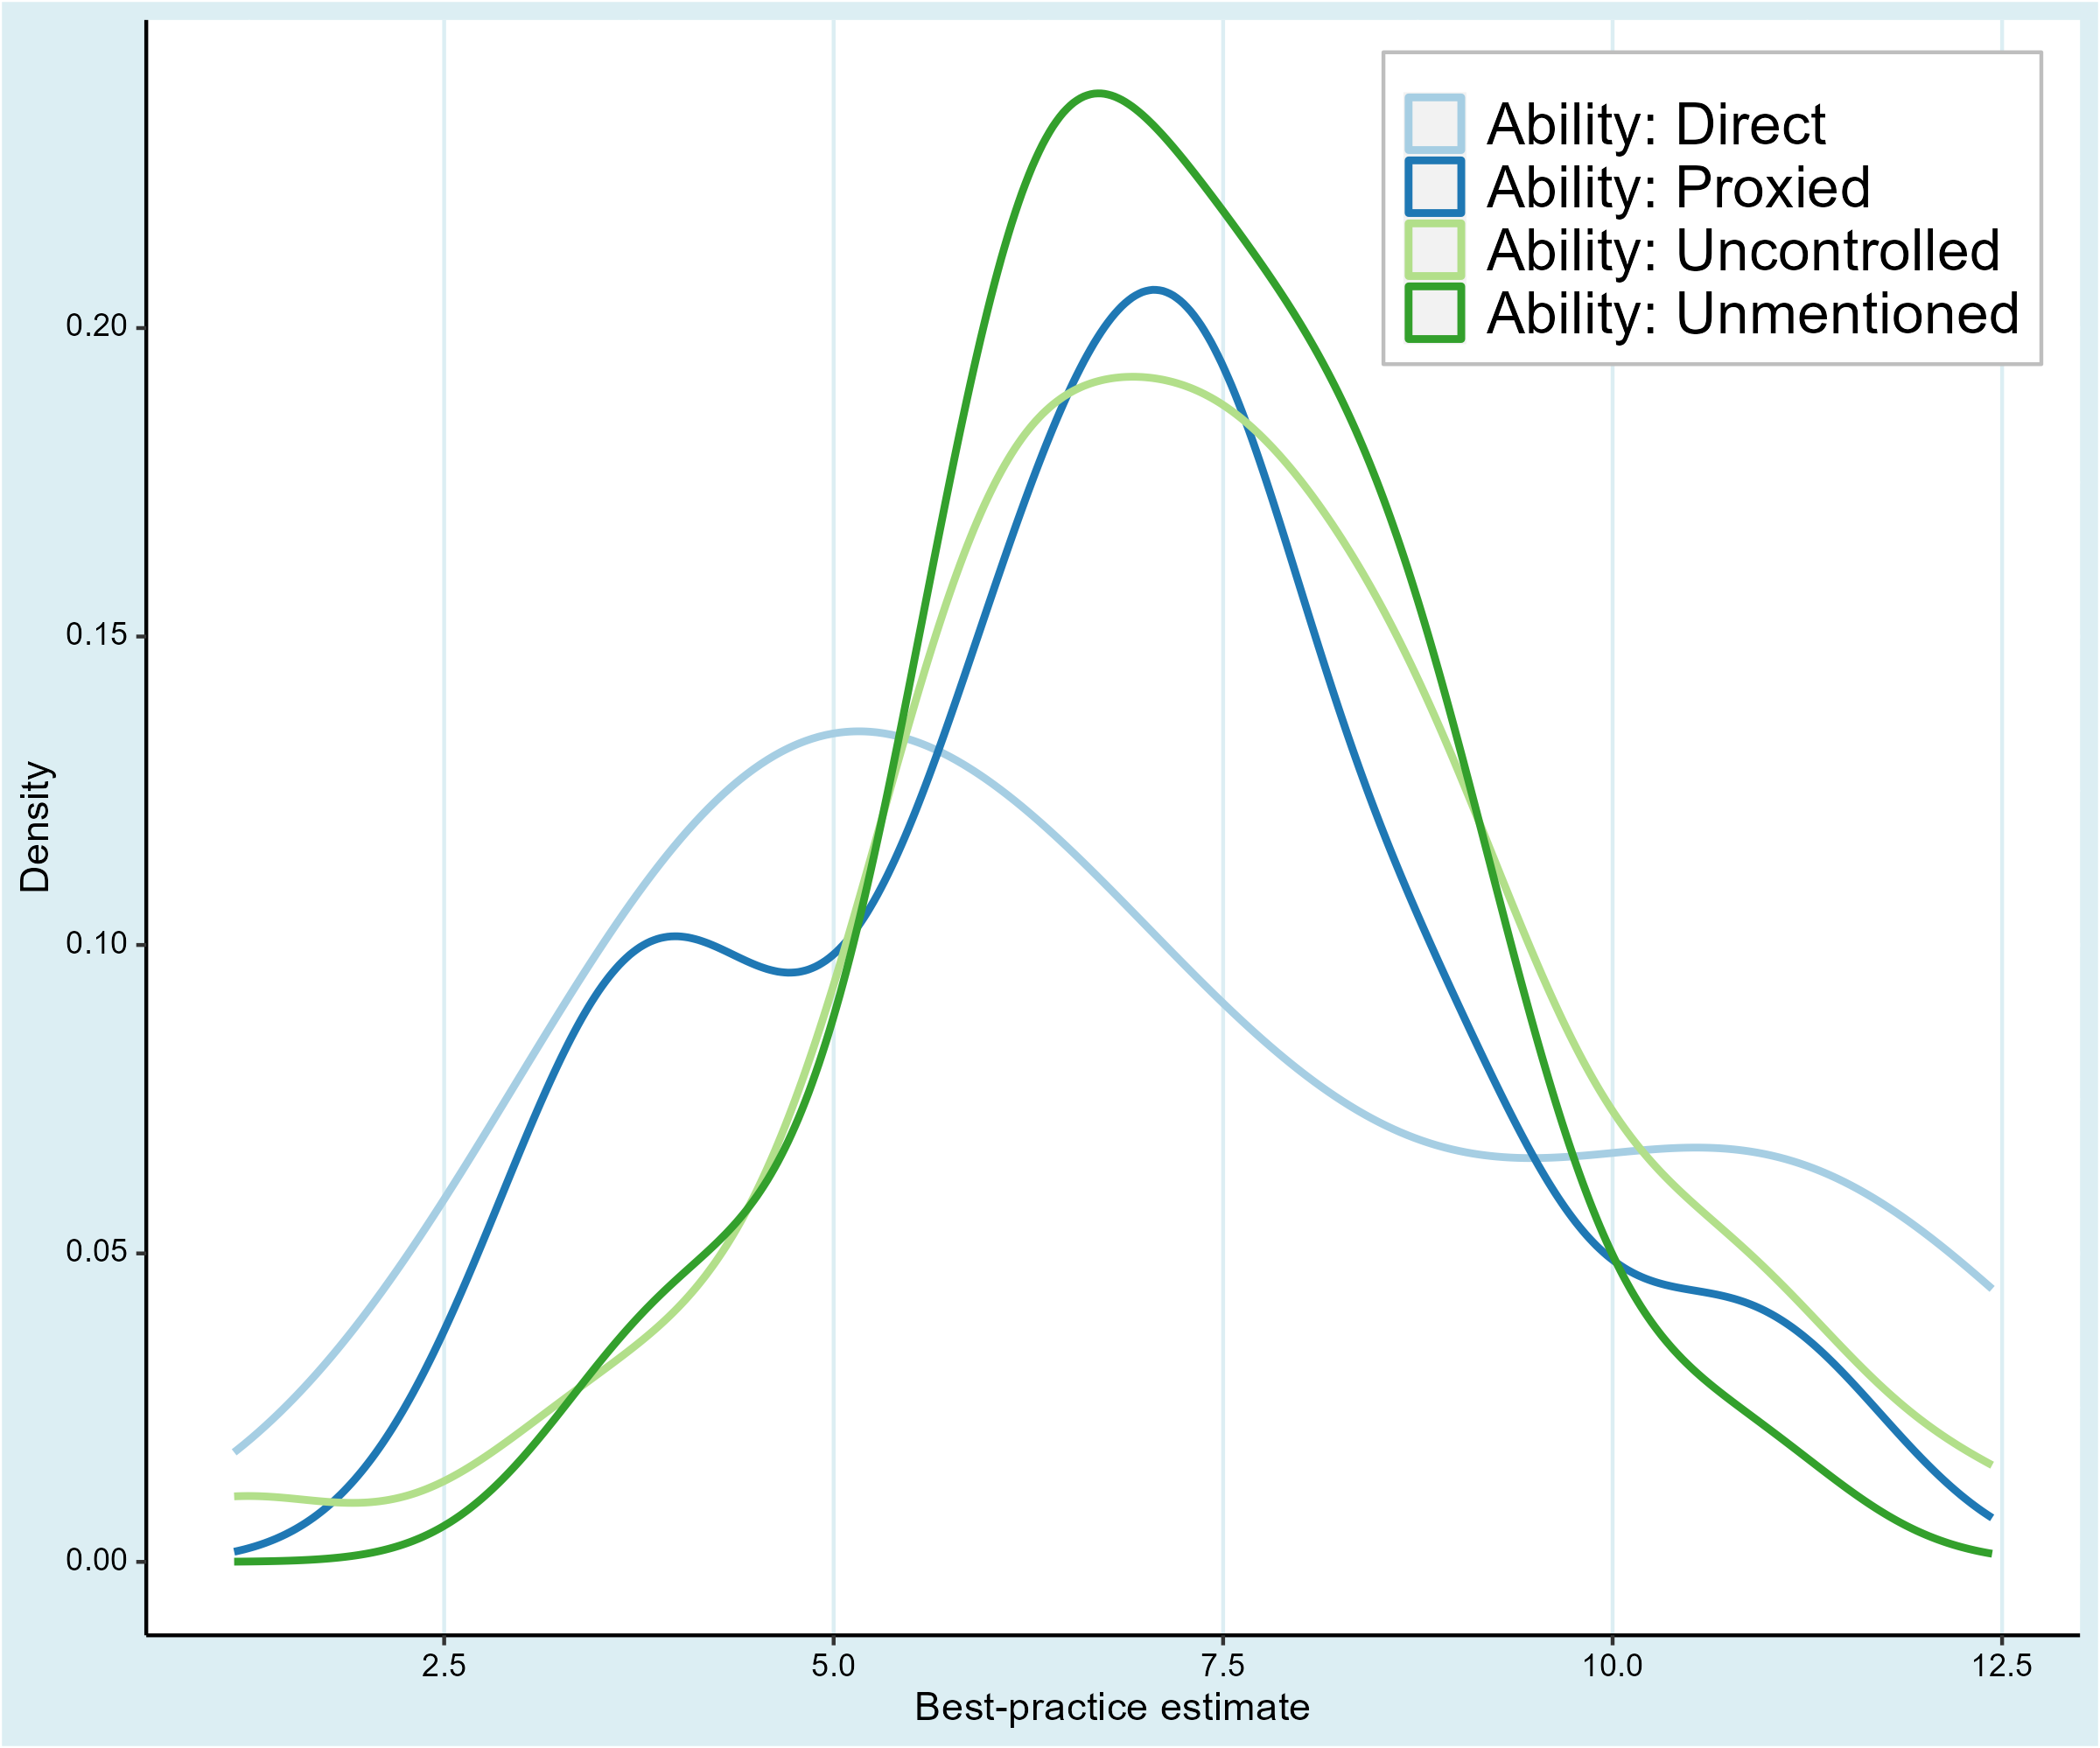
\includegraphics[width=0.95\linewidth]{Figures/BPE/bpe_ability.png}
      \label{fig:bpe_ability}
    \end{subfigure}
    \begin{subfigure}[!htbp]{0.38\textwidth}
      \vspace{0.2cm}
      \caption{Citations}
      \vspace{-0.1cm}
      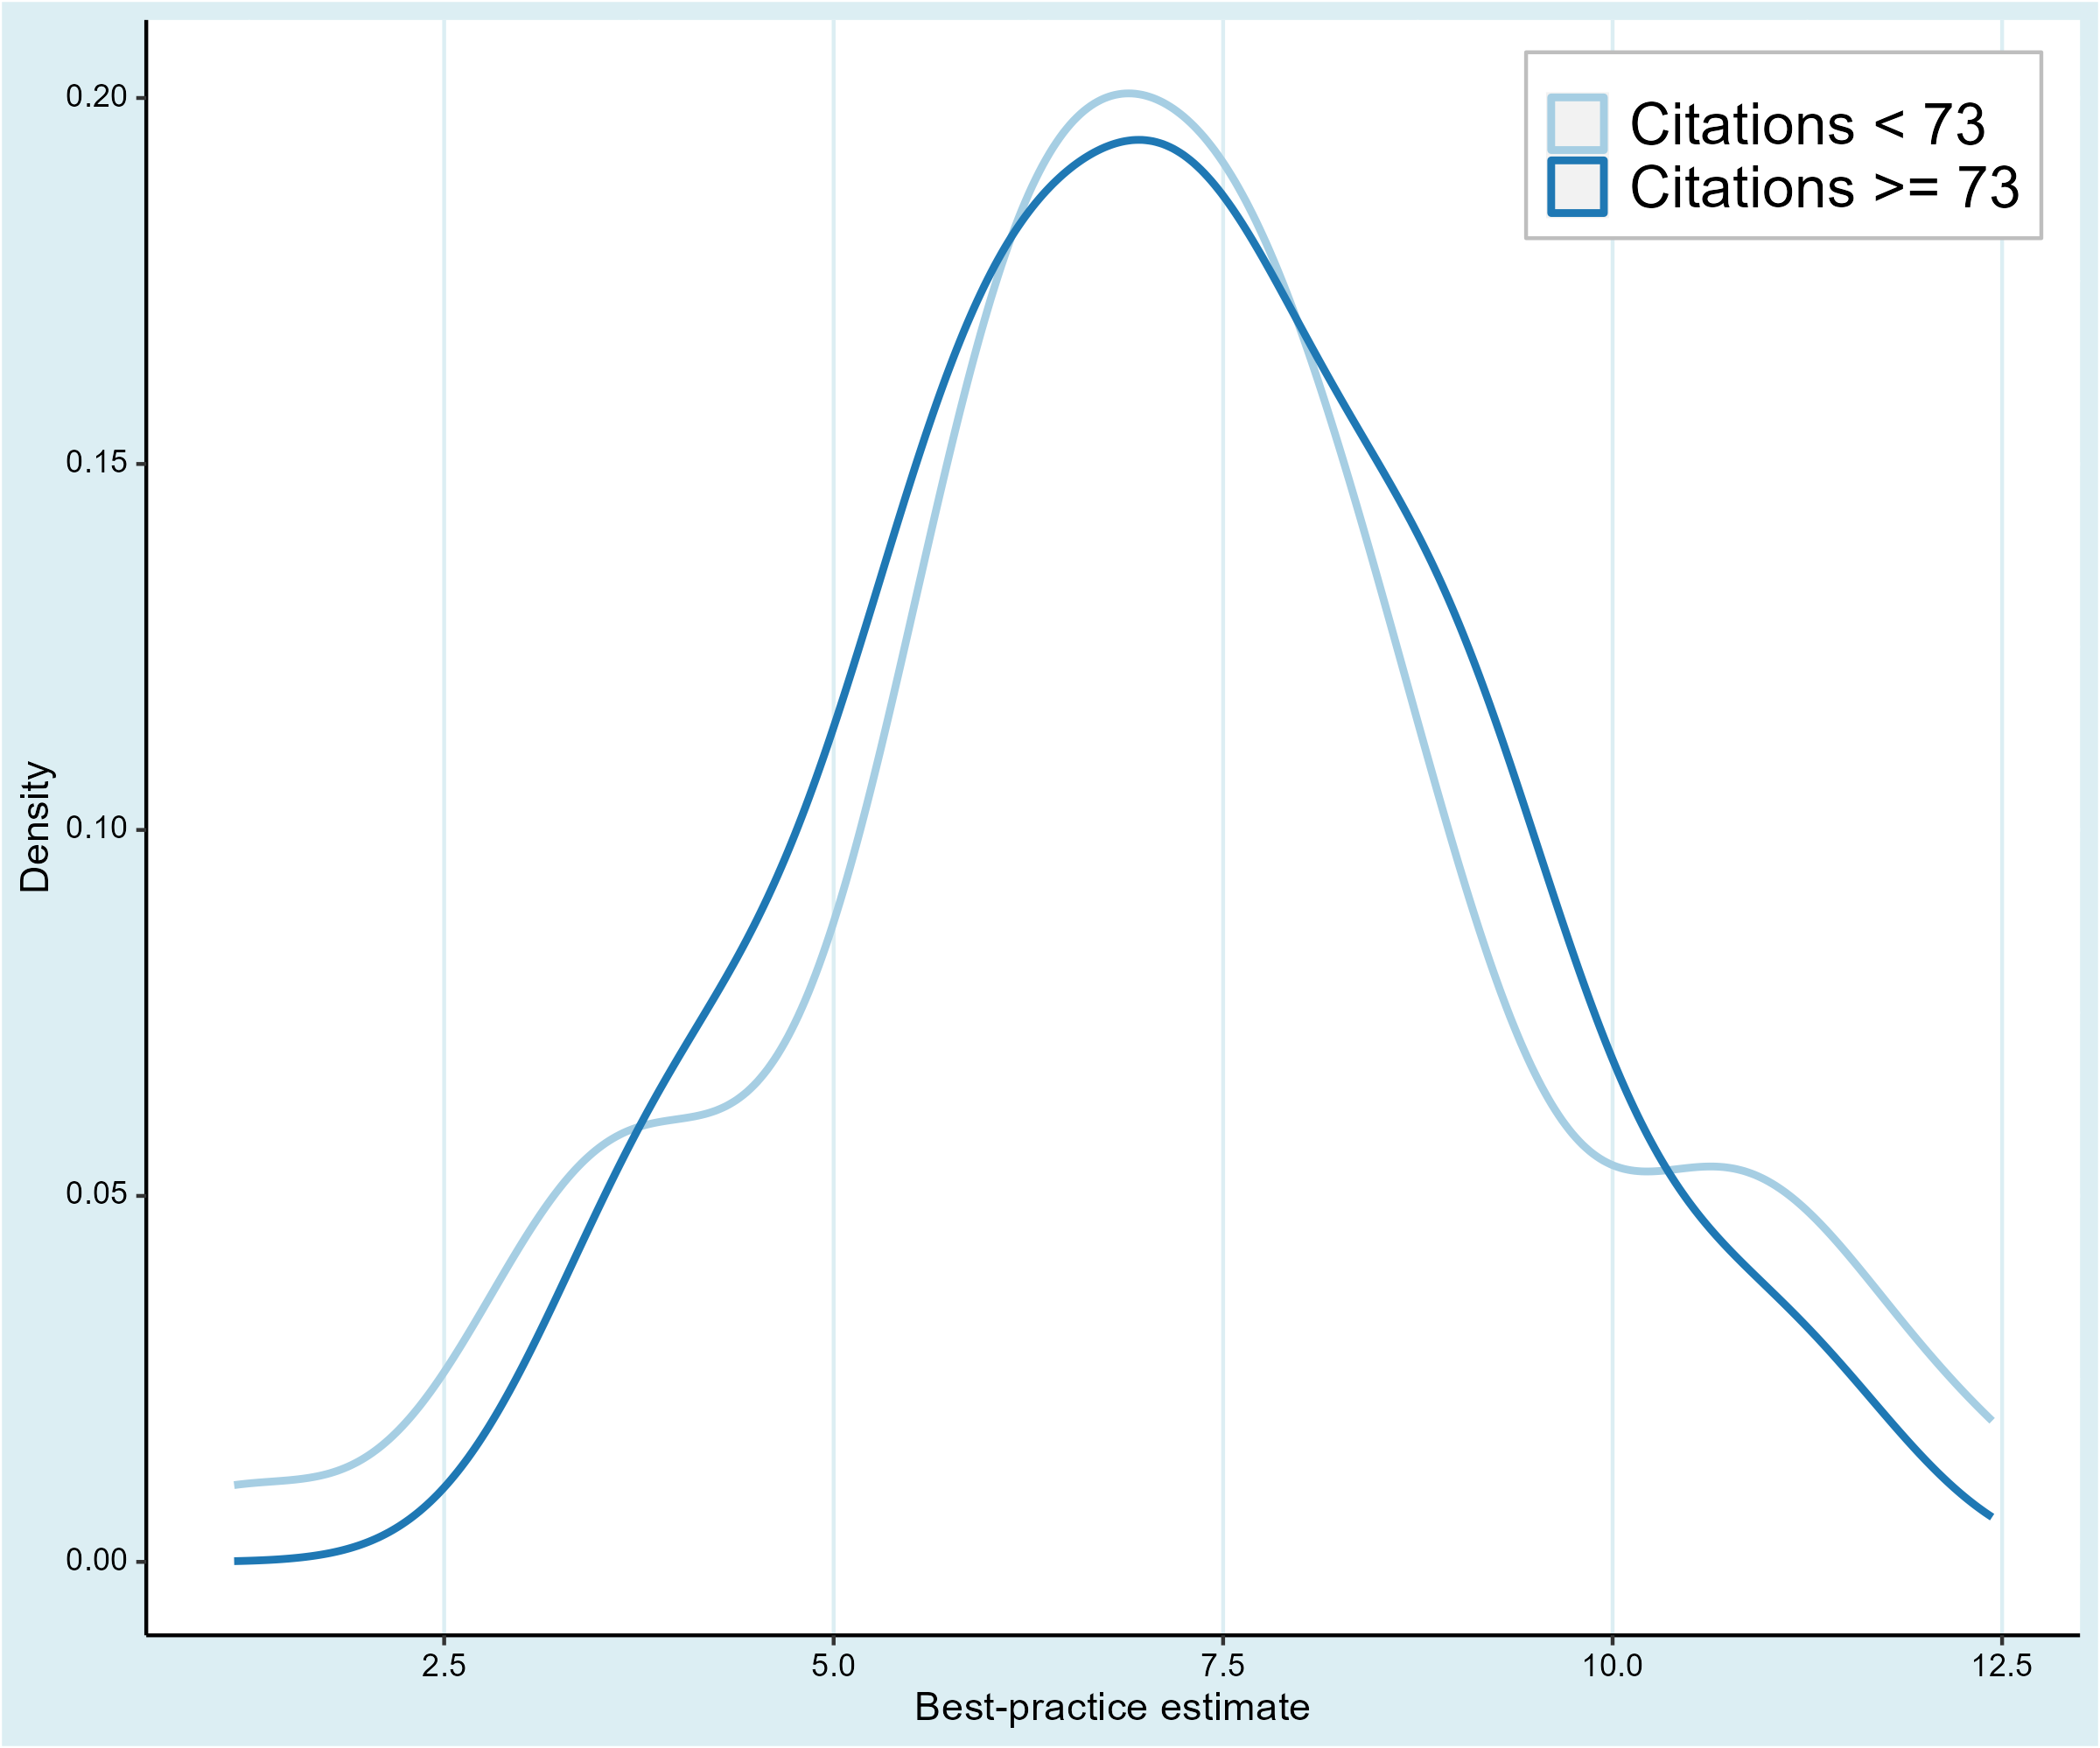
\includegraphics[width=0.95\linewidth]{Figures/BPE/bpe_citations.png}
      \label{fig:bpe_citations}
    \end{subfigure}

  \end{center}\vspace{-0.6cm}
  \captionsetup{width=0.78\textwidth, font = scriptsize}
  \caption*{\emph{Note:} This figure displays density lines for best-practice estimates of studies employing different variable setups. Each density line corresponds to a subset of studies whose setup involves a particular variable, as described in each graph's legend. The effect of an additional year of schooling on returns is displayed on the x-axis against its density on the y-axis. For \autoref{fig:bpe_citations}, the data median is used to determine the subsets. For a description of the variables used in these figures, see \autoref{tab:var}.}
\end{figure}

Several crucial points can be drawn from these graphs. First and foremost, it is vital to bear in mind the underlying large confidence interval with which these results are presented. Despite the lack of confidence bound curves in \autoref{fig:bpe_graphs}, the reader should bear in mind that the confidence range for these is quite wide. Second, as I pointed out earlier, some of these results are drawn from data subsets containing only a handful of studies, and should thus also be viewed with discretion, as they may be plagued with insufficient data sample bias. These include, but are not limited to, the subsamples of higher and primary education, low income countries, and several of the methodological subsamples.

% With the rate of 7.1\% returns to education as a baseline average of all best-practice estimates within the literature, some negative deviations appear for studies focusing on uneducated subjects (6.174\%), female subjects (6.388\%), studies employing cohort and fixed-effects estimation (5.861\%) or the Heckman method (6.417\%), and unpublished studies (6.535\%). Regarding ability, studies controlling for it directly or with a proxy report on average lower estimates (6.729\% and 6.873\%, respectively) than studies that omit ability from their models (7.134\% and 7.312\%). As for variables whose employment in study setup causes an increase in estimates, studies with subjects that attained higher education (7.729\%), or were self-employed (8.175\%), stand out among the rest. For the most part, even the differences in means are only marginal and amount to only one or two percentage points in returns at most.

With these considerations in mind, I dare to point out several intriguing patterns within the results. The left-hand side of distributions is visibly more prominent for studies focusing on female subjects, suggesting lower rate of returns to education associated with a greater amount of studies. A sizable bump of low percentage estimates also appears in the distribution of estimates for studies focusing on uneducated subjects. Still, due to the low number of studies in this subset, it is likely caused by an anomaly in one or two studies' calculations. The biggest takeaway from these results, however, should perhaps be unambiguous difference between the distributions of studies that control for ability (either directly or through a proxy), versus those who do not. The former group of studies displays a clear left skew, with the majority of estimates falling below the average of the whole literature. In contrast, the latter group of studies shows a right skew, with the majority of estimates falling above the average. This is in line with the results from \autoref{chap:four}, where I found that controlling for ability directly diminishes the overall effect, while leaving the ability out of the equation is associated with higher returns to education.

\section{Economic significance}
\label{sec:economic_significance}

Let us now return to the subjective best-practice estimate and consider the role of individual variables again. Namely, I will calculate the economic significance of some prominent variables, which means observing how much each of these variables contributes to the implied best practice when its value is changed. Variables with low \ac{PIP} in the model averaging could be argued to have little impact on the effect in the first place, so for this case, I will be considering only those variables that had \ac{PIP} at least 0.5. In the case of the \ac{BMA} model outlined in \autoref{chap:five}, that totals up to 19 variables. To determine their impact on the effect, I will calculate first how much the implied best-practice changes when there occurs a one standard deviation change in each variable, and then how much that change will be when the variable shifts from its lowest reported value to its highest. The results of these calculations can be found in \autoref{tab:econ_significance}.

% BPE Economic Significance
\begin{table}[!htbp]
  \centering
  \scriptsize
  \singlespace
  \caption{Economic significance of key variables}
  \label{tab:econ_significance}
  \begin{tabular}{
      @{}
      l
      *{4}{c}
      @{}}
    \toprule
                          & \multicolumn{2}{c}{One SD change} & \multicolumn{2}{c}{Maximum change}                                \\
                          & Effect on Returns                 & \% of BP                           & Effect on Returns & \% of BP \\
    \midrule
    Standard Error        & 0.635                             & 9.78\%                             & 3.399             & 52.37\%  \\
    Estimate: Sub-region  & -0.442                            & -6.81\%                            & -1.479            & -22.79\% \\
    Estimate: Region      & -0.616                            & -9.5\%                             & -1.334            & -20.55\% \\
    Education: Years      & 0.554                             & 8.53\%                             & 1.149             & 17.71\%  \\
    Wage: Log Hourly      & -0.216                            & -3.32\%                            & -0.432            & -6.66\%  \\
    Wage: Log Daily       & -0.472                            & -7.27\%                            & -1.611            & -24.81\% \\
    Wage: Log Monthly     & -0.274                            & -4.22\%                            & -0.671            & -10.34\% \\
    Micro Data            & 0.525                             & 8.09\%                             & 1.374             & 21.17\%  \\
    Primary Education     & 0.522                             & 8.04\%                             & 3.455             & 53.23\%  \\
    Higher Education      & 1.336                             & 20.58\%                            & 5.397             & 83.14\%  \\
    Wage Earners          & 0.181                             & 2.78\%                             & 0.882             & 13.59\%  \\
    Male                  & -0.420                            & -6.48\%                            & -1.202            & -18.51\% \\
    Ethnicity: Caucasian  & -0.612                            & -9.43\%                            & -1.460            & -22.49\% \\
    Method: 2SLS          & 0.449                             & 6.91\%                             & 1.529             & 23.55\%  \\
    Method: IV            & 0.832                             & 12.81\%                            & 2.651             & 40.84\%  \\
    Ability: Direct       & -0.416                            & -6.41\%                            & -1.218            & -18.77\% \\
    Ability: Uncontrolled & 0.243                             & 3.75\%                             & 0.492             & 7.58\%   \\
    Control: Age          & -0.913                            & -14.07\%                           & -1.921            & -29.6\%  \\
    Control: Age$^2$      & 1.336                             & 20.58\%                            & 2.992             & 46.1\%   \\
    Control: Area         & 0.880                             & 13.56\%                            & 1.784             & 27.48\%  \\
    Impact Factor         & -0.330                            & -5.08\%                            & -1.501            & -23.13\% \\
    Study: Published      & -0.491                            & -7.57\%                            & -1.157            & -17.82\% \\
    \bottomrule
    \multicolumn{5}{>{\scriptsize}p{0.8\linewidth}}{\emph{Note:}
    This table lists individual effects of variables on returns to schooling, ceteris paribus. Only varaibles identified as important (PIP $\geq$ 0.5) during the Bayesian Modal Averaging are listed. One SD change = How much the effect changes when the variable changes by one standard deviation. Maximum change = How much the effect changes when the variable changes from its lowest to its highest value. The variables are compared against a baseline of 6.536\% returns to education (author's subjective best-practice estimate). For an exmplanation of all the listed variables, refer to \autoref{tab:var}. SD = Standard deviation, 2SLS = Two-stage Least Squares, IV = Instrumental Variable.}
  \end{tabular}
\end{table}

With 6.536\% as the reference value of the effect against which the economic significance is compared, there are nine variables with negative influence. In contrast, ten variables pull the effect in the positive direction. Understandably, the standard error is among the variables with a positive sign (0.635 for 1 SD change, 3.399 for maximum change), as an increase in standard error should highly correlate to an increase in the effect. Otherwise, there would have been an unmistakable publication bias in the literature, which the tests in \autoref{chap:four} failed to provide conclusive evidence for. As for the rest of the variables, higher finished education, \ac{IV} regression, age in the quadratic form, and controlling for area display the highest positive impact among the rest. However, the coefficient for the age squared is offset by its linear counterpart, giving the expected convex shape to the Mincer equation and predicting a substantial increase in earnings later in life. Out of the other variables with positive direction, \textit{Education: Years} stands out the most, underlining the suspicion that estimates reporting education in highest achieved levels instead of in years tend to underestimate the returns to education.

As for the variables with a negative influence on the effect, the most significant change is associated with the aforementioned linear age coefficient. Apart from said coefficient, regional and sub-regional level estimates also diminish the overall effect, as does being a male or Caucasian ethnicity. Further, studies with a high impact factor or studies published in journals tend to report higher estimates than their less recognized counterparts. And last but not least, the issue of ability. As has been the case thus far, controlling for ability directly diminishes the overall effect, while leaving the ability out of the equation is associated with higher returns to education. The size of this ability bias, at least when looking at the economic significance of variables, is relatively smaller. Despite this, its presence is unmistakable and in line with all the results presented thus far.